% Options for packages loaded elsewhere
\PassOptionsToPackage{unicode}{hyperref}
\PassOptionsToPackage{hyphens}{url}
%
\documentclass[
]{article}
\usepackage{amsmath,amssymb}
\usepackage{iftex}
\ifPDFTeX
  \usepackage[T1]{fontenc}
  \usepackage[utf8]{inputenc}
  \usepackage{textcomp} % provide euro and other symbols
\else % if luatex or xetex
  \usepackage{unicode-math} % this also loads fontspec
  \defaultfontfeatures{Scale=MatchLowercase}
  \defaultfontfeatures[\rmfamily]{Ligatures=TeX,Scale=1}
\fi
\usepackage{lmodern}
\ifPDFTeX\else
  % xetex/luatex font selection
\fi
% Use upquote if available, for straight quotes in verbatim environments
\IfFileExists{upquote.sty}{\usepackage{upquote}}{}
\IfFileExists{microtype.sty}{% use microtype if available
  \usepackage[]{microtype}
  \UseMicrotypeSet[protrusion]{basicmath} % disable protrusion for tt fonts
}{}
\makeatletter
\@ifundefined{KOMAClassName}{% if non-KOMA class
  \IfFileExists{parskip.sty}{%
    \usepackage{parskip}
  }{% else
    \setlength{\parindent}{0pt}
    \setlength{\parskip}{6pt plus 2pt minus 1pt}}
}{% if KOMA class
  \KOMAoptions{parskip=half}}
\makeatother
\usepackage{xcolor}
\usepackage[margin=1in]{geometry}
\usepackage{longtable,booktabs,array}
\usepackage{calc} % for calculating minipage widths
% Correct order of tables after \paragraph or \subparagraph
\usepackage{etoolbox}
\makeatletter
\patchcmd\longtable{\par}{\if@noskipsec\mbox{}\fi\par}{}{}
\makeatother
% Allow footnotes in longtable head/foot
\IfFileExists{footnotehyper.sty}{\usepackage{footnotehyper}}{\usepackage{footnote}}
\makesavenoteenv{longtable}
\usepackage{graphicx}
\makeatletter
\def\maxwidth{\ifdim\Gin@nat@width>\linewidth\linewidth\else\Gin@nat@width\fi}
\def\maxheight{\ifdim\Gin@nat@height>\textheight\textheight\else\Gin@nat@height\fi}
\makeatother
% Scale images if necessary, so that they will not overflow the page
% margins by default, and it is still possible to overwrite the defaults
% using explicit options in \includegraphics[width, height, ...]{}
\setkeys{Gin}{width=\maxwidth,height=\maxheight,keepaspectratio}
% Set default figure placement to htbp
\makeatletter
\def\fps@figure{htbp}
\makeatother
\setlength{\emergencystretch}{3em} % prevent overfull lines
\providecommand{\tightlist}{%
  \setlength{\itemsep}{0pt}\setlength{\parskip}{0pt}}
\setcounter{secnumdepth}{5}
\newlength{\cslhangindent}
\setlength{\cslhangindent}{1.5em}
\newlength{\csllabelwidth}
\setlength{\csllabelwidth}{3em}
\newlength{\cslentryspacingunit} % times entry-spacing
\setlength{\cslentryspacingunit}{\parskip}
\newenvironment{CSLReferences}[2] % #1 hanging-ident, #2 entry spacing
 {% don't indent paragraphs
  \setlength{\parindent}{0pt}
  % turn on hanging indent if param 1 is 1
  \ifodd #1
  \let\oldpar\par
  \def\par{\hangindent=\cslhangindent\oldpar}
  \fi
  % set entry spacing
  \setlength{\parskip}{#2\cslentryspacingunit}
 }%
 {}
\usepackage{calc}
\newcommand{\CSLBlock}[1]{#1\hfill\break}
\newcommand{\CSLLeftMargin}[1]{\parbox[t]{\csllabelwidth}{#1}}
\newcommand{\CSLRightInline}[1]{\parbox[t]{\linewidth - \csllabelwidth}{#1}\break}
\newcommand{\CSLIndent}[1]{\hspace{\cslhangindent}#1}
\usepackage{caption}
\captionsetup[figure]{font=small}
\usepackage{lineno}
\linenumbers
\usepackage{flafter}
\usepackage{booktabs}
\usepackage{longtable}
\usepackage{array}
\usepackage{multirow}
\usepackage{wrapfig}
\usepackage{float}
\usepackage{colortbl}
\usepackage{pdflscape}
\usepackage{tabu}
\usepackage{threeparttable}
\usepackage{threeparttablex}
\usepackage[normalem]{ulem}
\usepackage{makecell}
\usepackage{xcolor}
\ifLuaTeX
  \usepackage{selnolig}  % disable illegal ligatures
\fi
\IfFileExists{bookmark.sty}{\usepackage{bookmark}}{\usepackage{hyperref}}
\IfFileExists{xurl.sty}{\usepackage{xurl}}{} % add URL line breaks if available
\urlstyle{same}
\hypersetup{
  pdftitle={Meta-Analysis of Variation in Sport and Exercise Science},
  hidelinks,
  pdfcreator={LaTeX via pandoc}}

\title{Meta-Analysis of Variation in Sport and Exercise Science}
\usepackage{etoolbox}
\makeatletter
\providecommand{\subtitle}[1]{% add subtitle to \maketitle
  \apptocmd{\@title}{\par {\large #1 \par}}{}{}
}
\makeatother
\subtitle{Examples of Application Within Resistance Training Research}
\author{}
\date{14th September 2023}

\begin{document}
\maketitle
\begin{abstract}
Meta-analysis has become commonplace within sport and exercise science for synthesising and summarising empirical studies. However, most research in the field focuses upon mean effects; particularly the effects of interventions to improve outcomes such as fitness or performance. It is thought that \textcolor{red}{individual responses to interventions vary considerably}. Hence, interest has increased in exploring \emph{precision} or \emph{personalised} exercise approaches. Not only is the mean often affected by interventions, but variances may also be impacted. Exploration of variances in studies such as randomised controlled trials (RCTs) can yield insight into interindividual heterogeneity in response to interventions and help determine generalisability of effects. Yet, larger samples sizes than those used for typical mean effects are required when probing variances. Thus, \textcolor{red}{in} a field with small samples such as sport and exercise science, exploration of variance through a meta-analytic framework is appealing. \textcolor{red}{Despite} the value of embracing and exploring variation alongside mean effects in sport and exercise science \textcolor{red}{it is rarely applied to research synthesis through meta-analysis}.\textcolor{red}{We introduce and evaluate different effect size calculations along with models for meta-analysis of variation using relatable examples from resistance training RCTs}.
\end{abstract}

\hypertarget{introduction}{%
\section{Introduction}\label{introduction}}

Although the quantitative synthesis of results across studies has existed since the 17th century (Plackett, 1958), the modern-day term ``meta-analysis'' was coined by Gene Glass (1976). Since that time, the use of meta-analysis as a tool for the synthesis of research in sport and exercise science has increased considerably (Hagger, 2022), with resistance training (RT) accounting for a considerable proportion of this growth (figure @ref(fig:trend-plot)). Accordingly, throughout the paper we use RT studies as a hopefully familiar example for sport and exercise science researchers. \textcolor{red}{However, to begin we provide a conceptual overview of meta-analyses and effect sizes as typically used within sport and exercise science.}

\begin{figure}

{\centering 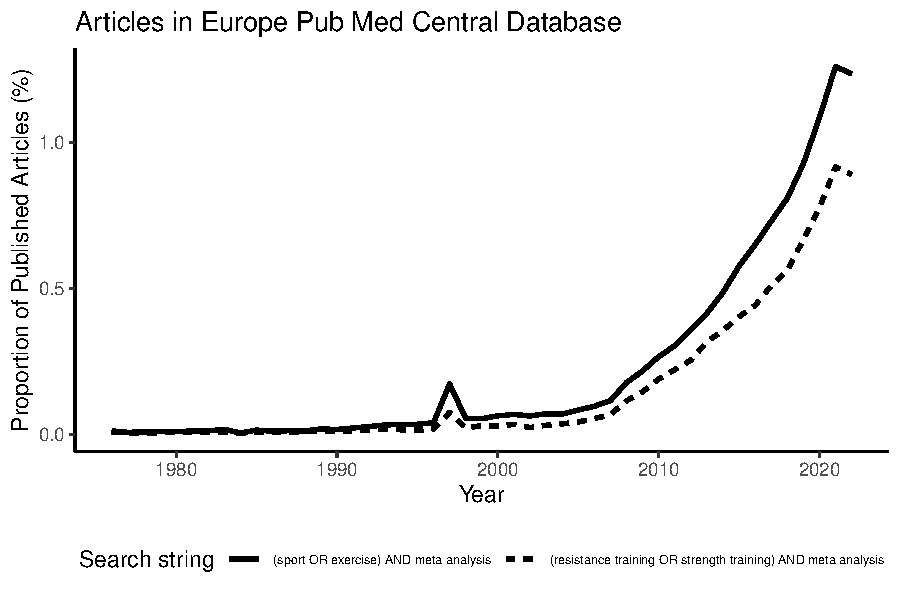
\includegraphics{Revised-Paper---Meta-Analysis-of-Variation-in-Sport-and-Exercise-Science---anonymous_files/figure-latex/trend-plot-1} 

}

\caption{Trends in meta-analyses published in sport and exercise science since 1976.}(\#fig:trend-plot)
\end{figure}

\textcolor{red}{There are two popular models}\footnote{\textcolor{red}{To clarify language here for those unfamiliar, the term and concept *model* is used commonly in statistics. A statistical model essentially is specification of what we think the data generating process might be for a given situation. In the context of meta-analyses the data are usually the individual effects that we have extracted from studies i.e., the results of each study. The model, in mathematical formulae, is intended to approximate the processes that we assume led to the generation of the data.}} \textcolor{red}{used for meta-analysis: the fixed-effect model and the random-effects model} (Borenstein et al., 2010). \textcolor{red}{The fixed effect model assumes that there is one true effect size}\footnote{\textcolor{red}{*Effect size* is an agnostic term used for a family of statistics which communicate the strength of a given 'effect' resulting from research. This includes descriptive statistics ranging from mean raw values to correlation coeffients and everything in between} (Caldwell \& Vigotsky, 2020) \textcolor{red}{including, as we shall see, statistics describing variation.}} \textcolor{red}{that each study included in the meta-analysis has estimated and that any differences in the estimates between individual studies are due to only sampling error. This essentially means that there is a single common effect which is fixed across studies and each study takes samples of individuals from the population to estimate this effect. We can express this model in the following formula:}

\begin{equation}
\hat\theta_{i}=\theta+m_{i} 
(\#eq:fixed-model-eq)
\end{equation}

\textcolor{red}{where $\hat\theta_{i}$ is the $i\textrm{th}$ effect size ($i = 1,2,\cdots,N_{i}$; where $N_{i}$ is the number of studies and thus effect sizes), $\theta$ is the intercept or overall mean (i.e., the fixed-effect), and $m_{i}$ is the sampling error for each effect size normally distributed with $\sigma^2_{m_{i}}$. Studies with smaller standard errors of their effect estimates have smaller sampling errors and so these higher precision estimates are given greater weight in the model. The weighting given to each study is calculated as:}

\begin{equation}
w_{i}=\frac{1}{s^2_{i}}
(\#eq:fixed-weights-eq)
\end{equation}

\textcolor{red}{Where $s_{i}$ is the standard deviation for the effect estimate and thus $s^2_{i}$ is the variance. It is referred to as inverse-variance weighting. Then, the overall weighted mean effect estimate from the model is then calculated as:}

\begin{equation}
\hat\theta=\frac{\sum^I_{i=1}\hat\theta_{i}w_{i}}{\sum^I_{i=1}w_{i}}
(\#eq:fixed-average-eq)
\end{equation}

\textcolor{red}{Contrastingly, the random effects model does not make the assumption that there is only one fixed-effect. Instead it allows for the true effects that each study estimates to differ. Each study may share a common underlying effect size but, due to differences between studies in factors such as population characteristics, the manner in which outcomes are operationalised, or subtle differences in intervention and context to name a few, it is possible that the actual effect being estimated by each study differs. The assumption of the random-effects model then is that the studies included estimate effects that come from a larger population of effects determined by the inclusion criteria for studies included. So, the model assumes that the studies included reflect a random sample of all possible permutations of study and the effects they estimate from this population distribution of studies and effects. Hence, in the fixed-effect model there is one effect and it is assumed to be *fixed* across studies, whereas in the random-effects model there are many and we examine an assumed *random* sample of them. We can express this model in the following formula:}

\begin{equation}
\hat\theta_{i}=\theta_{i}+\tau_{i}+m_{i}
(\#eq:random-model-eq)
\end{equation}

\textcolor{red}{where $\hat\theta_{i}$ is the $i\textrm{th}$ effect size ($i = 1,2,\cdots,N_{i}$; where $N_{i}$ is the number of studies and thus effect sizes), $\theta_i$ is the intercept or overall mean of the effects across each study, $\tau_{i}$ is the deviation from $\theta_{i}$ for the $i\textrm{th}$ study (i.e., the random-effects), and $m_{i}$ is the sampling error for each effect size normally distributed with $\sigma^2_{m_{i}}$. Essentially this model assumes that each individual study estimates an effect and there will be some sampling error in estimating it. But, the effects each study estimates comes from an overall distribution of true effects with a mean value (i.e., $\theta_{i}$). The weighting in any model employing random effects such as this requires a different approach as the variance of the distribution of the effect sizes the model assumes, known as $\tau^2$, must also be estimated}\footnote{\textcolor{red}{This estimation can be done using a variety of methods and is an area of ongoing investigation as to how different methods perform. This is beyond the scope of this paper to discuss. We note however that the models we present all utilise Restricted Maximum Likelihood estimation.}}. \textcolor{red}{This essentially describes the heterogeneity between the effects included. Once this has been estimated we can calculate a weight that is adjusted for the random effects for each effect as:}

\begin{equation}
w^*_{i}=\frac{1}{s^2_{i}+\tau^2}
(\#eq:random-weights-eq)
\end{equation}

\textcolor{red}{Then the average of the distribution of effects can be calculated as per equation} @ref(eq:fixed-average-eq) \textcolor{red}{substituting $w_{i}$ for $w^*_{i}$.}

\textcolor{red}{Although historically fixed effect models were commonplace in the field of sport and exercise science} (Hagger, 2006) \textcolor{red}{nowadays the random effects model is more often employed} (Hagger, 2022). \textcolor{red}{This is likely due to the fact that direct (i.e., exact) replication of studies is rare}\footnote{\textcolor{red}{Hence current efforts to conduct direct replications (see https://ssreplicationcentre.com/).}} \textcolor{red}{and instead studies often explore similar effects across varying moderating factors such as those noted above.}

As with many other fields (Mills et al., 2021; Nakagawa et al., 2015; Usui et al., 2021) \textcolor{red}{likely the most common aim in meta-analysis in sport and exercise science, and indeed primary empirical research too, is to estimate the *effect* of an independent variable upon some dependent outcome variable. The dependent variable is often the mean of a measurement and the independent variable is often a categorical grouping}; for example, the comparison of an intervention group(s) and a control group, the comparison of intervention groups between one another, or comparison between non-manipulated categories such as biological sex. Indeed, a recent umbrella review (Bernárdez-Vázquez et al., 2022) of meta-analyses in RT identified 14 studies examining the manipulation of RT intervention variables (i.e., the comparison of one intervention to another whereby a variable in the intervention was manipulated) on hypertrophy outcomes, all of which focused on the comparison of mean changes between different intervention groups.

\textcolor{red}{Often, due to the varying operationalisations used for broad outcome concepts}\footnote{\textcolor{red}{For example, *strength* might be examined in different studies using different operationalisations including one repetition maximum testing or maximum voluntary contractions. Or the same operationalisations may be employed but different exercises such as the squat or bench press.}}\textcolor{red}{, an effect size is used which is "standardised" across studies to allow for their synthesis.} Most commonly, a magnitude based\footnote{Though notably not all meta-analyses use \emph{magnitude based} effect sizes. Indeed some explicitly use what Caldwell and Vigotsky (2020) term \emph{signal-to-noise} effect sizes (e.g., Heidel et al. (2022)).} effect size statistic (Caldwell \& Vigotsky, 2020), the standardised mean difference (SMD), is used to compare means between groups or conditions. This statistic is usually a version of Cohen's \emph{d} (Cohen, 1988), or its bias-corrected\footnote{\textcolor{red}{For those unfamiliar with the terminology, an estimator for a statistic is unbiased if it produces parameter estimates that are on average correct. Thus a bias corrected statistic is one which would be biased without the correction applied, but otherwise has been shown to be unbiased.}} metric referred to as Hedges' \emph{g} {[}Hedges \& Olkin (2014); Borenstein et al. (2021); Nakagawa \& Cuthill (2007){]}\footnote{We will refer to both merely as the SMD throughout the manuscript for simplicity and note that throughout when reporting a `SMD' we are reporting the bias-corrected version. \textcolor{red}{We also note that another magnitude based effect size, Glass' $\Delta$, is commonly recommended as it is the simplest form of SMD though makes assumptions about the impact of the intervention having no effect on the denominator (i.e., variance;} Caldwell \& Vigotsky (2020)).}. The SMD, and its sampling variance, \(s^2_{SMD}\) are given by:

\begin{equation}
SMD=\frac{\overline{x}_E - \overline{x}_C}{s_{pooled}}J
(\#eq:SMD-eq)
\end{equation}

\begin{equation}
J=1-\frac{3}{4(n_{C}+n_{E})-2)-1}
(\#eq:biasJ-eq)
\end{equation}

\begin{equation}
s_{pooled}=\sqrt{\frac{(n_{C}-1)s^2_{C}+(n_{E}-1)s^2_{E}}{n_{C}+n_{E}-2}}
(\#eq:s-pooled-eq)
\end{equation}

\begin{equation}
s^2_{SMD}=\frac{n_{C}+n_{E}}{n_{C}n_{E}}+\frac{SMD^2}{2(n_{E}+n_{C})}
(\#eq:SMDvar-eq)
\end{equation}

where \(\overline{x}_C\) and \(\overline{x}_E\) are the sample means of the control group (C) and experimental (E) or intervention group respectively, \(s_C\) and \(s_E\) are the standard deviations of the two groups, \(n_C\) and \(n_E\) are the sample sizes of the two groups, and \(J\) is a bias correction for small sample sizes.

The natural logarithm of the ratio of two means (\(\textrm{ln}RR\)) is also another effect size statistic that can be used (Curtis \& Wang, 1998; Hedges et al., 1999; Lajeunesse, 2011, 2015). The lnRR, and its sampling variance, \(s^2_{\textrm{ln}RR}\) are given by:

\begin{equation}
\textrm{ln}RR=\textrm{ln}\frac{\overline{x}_E}{\overline{x}_C}
(\#eq:lnRR-eq)
\end{equation}

\begin{equation}
s^2_{\textrm{ln}RR}=\frac{s^2_{C}}{n_{C}\overline{x}^2_{C}}+\frac{s^4_{C}}{2n_{C}\overline{x}^2_{C}\overline{x}^4_{C}}+\frac{s^2_{E}}{n_{E}\overline{x}^2_{E}}+\frac{s^4_{E}}{2n_{E}\overline{x}^2_{E}\overline{x}^4_{E}}
(\#eq:lnRRvar-eq)
\end{equation}

Due to its calculation the SMD is affected not only by the difference in means of the two groups, but also by the standard deviations of both groups due to the standardisation of the effect size by \(s_{pooled}\) in the denominator. In contrast, the \(\textrm{ln}RR\) is uninfluenced by the standard deviations in either groups (see equation @ref(eq:lnRR-eq)), which only affects the sampling variance (see equation @ref(eq:lnRRvar-eq)). Despite this, the use of effect sizes like the \(\textrm{ln}RR\) has been limited in previous meta-analyses in sport and exercise science (Deb et al., 2018; Nuzzo et al., 2023a) and to our knowledge only a couple of meta-analyses of RT interventions has used this kind of effect size (Swinton et al., 2022; Wolf et al., 2023).

Although researchers in sport and exercise science, among other fields, have focused on estimating the average effects of interventions using randomised trial designs for both primary research and synthesis through meta-analysis, responses to certain interventions may vary on a subgroup or even individual basis. The increased interest in \emph{precision} or \emph{personalised} approaches to exercise prescription has resulted in a number of opinion and methodological review articles discussing statistical approaches to understanding interindividual response heterogeneity to exercise interventions (Atkinson et al., 2019; Atkinson \& Batterham, 2015; Hecksteden et al., 2015; Hopkins, 2015; Hrubeniuk et al., 2022; Kelley, 2022; Pickering \& Kiely, 2019; Ross et al., 2019; Swinton et al., 2018). However, despite the availability of approaches to compare variances between groups, in sport and exercise science this is rarely explored in primary research (Bonafiglia et al., 2022). Moreover, although there has been increased interest in recent years, few meta-analyses in sport and exercise include both comparisons of means and variances or explicitly aim to investigate the latter (Bonafiglia et al., 2022; Esteves et al., 2021; Fisher et al., 2022; Kelley et al., 2020, 2022; Steele et al., 2021). Examination of interindividual heterogeneity in response to interventions presents considerable value to researchers and practitioners in sport and exercise science; interventions with low interindividual variation are likely to be widely generalisable, whilst an intervention with high interindividual variation is likely to have effects that are either subgroup or individual specific. The former kind of intervention might be widely applicable across individuals, whilst the latter kind of intervention requires specific research, typically with large samples (Hecksteden et al., 2015), to tease out subgroup- or participant-by-intervention interactions to facilitate successful practical application.

Comparison of heterogeneity in responses, such as post-scores or change scores to interventions, are not the only possible use of statistical methods for comparing variances. For example, in other fields such as ecology there have been calls to shift focus of analysis onto the exploration of dispersion of traits between groups in non-experimental or intervention designs (Nakagawa \& Schielzeth, 2012). Some recent examples from sport and exercise science, and RT in particular, include primary research exploring between-participant acute response variation for the purposes of identifying methods\footnote{Exploration of methodological approaches and their impact on heterogeneity have also been explored in preclinical research (Usui et al., 2021).} to reduce RT stimulus heterogeneity, (Exner et al., 2022) as well as a meta-analysis exploring between-participant heterogeneity of accuracy in predicting proximity to task failure during RT (Halperin et al., 2022) \textcolor{red}{and in the number of repetitions that can be performed at different percentages of one repetition maximum} (Nuzzo et al., 2023b).

Given the value of embracing and exploring variation alongside mean effects in sport and exercise science, yet the lack of application in research synthesis by way of primary research or meta-analysis, we present and discuss effect size approaches and models for meta-analysis of variation. Indeed, meta-analysis presents a very valuable method for exploring variation in a field such as sport and exercise science due to the typically small samples in primary studies. Such small samples have even lower statistical power to detect differences in variation as compared to means (Yang et al., 2022).

\textcolor{red}{Although ultimately we will recommend the thoughtful consideration of assumptions for certain approaches regarding what effect size statistics and models to employ in examining variation through use of meta-analysis, we provide examples throughout using all approaches described in order to aid the reader in understanding their strengths and weaknesses. We hope this will make clear why we offer such recommendations in our discussion and conclusion. As we have up to this point, we will also make an effort to both present the mathematical formulations of the models described, as well as to provide an explanation of them in plain English.}

\hypertarget{effect-size-statistics-for-meta-analytic-comparisons-of-variation}{%
\section{Effect size statistics for meta-analytic comparisons of variation}\label{effect-size-statistics-for-meta-analytic-comparisons-of-variation}}

Until recent years there has been a dearth of effect size statistics available for the examination of variation in a meta-analytic framework. However, several have been proposed that we now describe: the standard deviation for individual responses (\(SD_{ir}\); Hopkins (2015); Atkinson \& Batterham (2015); Atkinson et al. (2019)), the log ratio of standard deviations (\(\textrm{ln}VR\); termed the ``variability ratio''; Hedges \& Nowell (1995)), and the log ratio of coefficient of variation (\(\textrm{ln}CVR\); termed the ``coefficient of variation ratio''; Nakagawa et al. (2015); Senior et al. (2020)). We present the independent groups versions due to use of randomised controlled trials in our examples below, but note that dependent versions (i.e., for comparing related samples) also exist for \(\textrm{ln}VR\) and \(\textrm{ln}CVR\) (Senior et al., 2020).

\hypertarget{standard-deviation-for-individual-responses-sd_ir}{%
\subsection{\texorpdfstring{Standard deviation for individual responses (\(SD_{ir}\))}{Standard deviation for individual responses (SD\_\{ir\})}}\label{standard-deviation-for-individual-responses-sd_ir}}

In the context of \emph{precision} or \emph{personalised} approaches to exercise prescription the \(SD_{ir}\) has been proposed as an approach to determine the extent to which individual responses manifest by comparison of variation between two groups; control and intervention (Atkinson et al., 2019; Atkinson \& Batterham, 2015; Hopkins, 2015). The standard deviation of change scores (post-intervention scores minus pre-intervention scores) within the intervention group reflects the gross combination of a number of sources of variation including: participant-by-intervention interactions (i.e., actual individual responsiveness or `trainability'), within-participant variability in intervention response (i.e., variability in response to the same intervention administered to the same participant), and random error (i.e., from pre and post measurements; Hecksteden et al. (2015)). The standard deviation of change scores from the control group (assuming it is a non-intervention control group and not something like a `usual-care' group) by contrast is assumed to only reflect random error\footnote{Though notably, in the case of health behaviour studies it may be the case that if someone volunteers for a study it could conceivably motivate them to alter various habits even when they are assigned to a control group thus influencing change scores.} (Hecksteden et al., 2015). As such, the difference in these standard deviations can be used to determine the extent to which additional variation has been introduced by the intervention and that might reflect individual responses. Whilst the \(SD_{ir}\) has been proposed and used primarily in the context of individual response variation to interventions, it should be noted that this kind of absolute comparison of variance between groups or conditions is not limited to such applications.

The \(SD_{ir}\), and its sampling variance, \(s^2_{SD_{ir}}\) are given by:

\begin{equation}
SD_{ir}=\sqrt{s^2_{E} - s^2_{C}}
(\#eq:SDir-eq)
\end{equation}

\begin{equation}
s^2_{SD_{ir}}=2\biggl(\frac{s^4_{E}}{n_{E}-1}+\frac{s^4_{C}}{n_{C}-1}\biggl)
(\#eq:sdIRvar-eq)
\end{equation}

Thus, the \(SD_{ir}\) reflects a comparison of the absolute variance in change scores between control and intervention groups. However, a potential concern with the \(SD_{ir}\) is its potential to violate assumptions of normality, which is not the case for other effect size statistics such as \(\textrm{ln}VR\) and \(\textrm{ln}CVR\).

\hypertarget{log-ratio-of-standard-deviations-textrmlnvr}{%
\subsection{\texorpdfstring{Log ratio of standard deviations (\(\textrm{ln}VR\))}{Log ratio of standard deviations (\textbackslash textrm\{ln\}VR)}}\label{log-ratio-of-standard-deviations-textrmlnvr}}

A similar effect size statistic for the comparison of absolute variance between groups, and one that has had wide applications in more than just intervention response variability within fields such as ecology and evolution, is the \(\textrm{ln}VR\) (Hedges \& Nowell, 1995; Nakagawa et al., 2015; Senior et al., 2020). An unbiased estimator of the natural logarithm of a population standard deviation (\(\textrm{ln}\sigma\)), and its sampling variance, \(s^2_{\textrm{ln}\sigma}\) is given by:

\begin{equation}
\textrm{ln}\hat\sigma=\textrm{ln}s+\frac{1}{2(n-1)}
(\#eq:lnsigma-eq)
\end{equation}

\begin{equation}
s^2_{\textrm{ln}\hat\sigma}=\frac{1}{2(n-1)}
(\#eq:lnsigmavar-eq)
\end{equation}

where \(\textrm{ln}\hat\sigma\) is an estimate of \(\textrm{ln}\sigma\), and it is assumed with sufficiently large sample size and value of \(\sigma\) that \(\textrm{ln}\sigma\) is normally distributed with variance \(s^2_{\textrm{ln}\sigma}\). Given equations @ref(eq:lnsigma-eq) and @ref(eq:lnsigmavar-eq), the logarithm of the ratio of standard deviations of two groups, such as a control and intervention, the \(\textrm{ln}VR\), and its sampling variance, \(s^2_{\textrm{ln}VR}\) is given by:

\begin{equation}
\textrm{ln}VR=\textrm{ln}\biggl(\frac{s_{E}}{s_{C}}\biggl)+\frac{1}{2(n_{E}-1)}-\frac{1}{2(n_{C}-1)}
(\#eq:lnVR-eq)
\end{equation}

\begin{equation}
s^2_{\textrm{ln}VR}=\frac{1}{2}\biggl(\frac{n_{C}}{(n_{C}-1)^2}+\frac{n_{E}}{(n_{E}-1)^2}\biggl)
(\#eq:lnVRvar-eq)
\end{equation}

However, due to both \(SD_{ir}\) and \(\textrm{ln}VR\) being comparisons of absolute variance, they may find limited applicability where the mean of one group is larger than the comparison group (e.g., when \(\overline{x}_E\) is larger than \(\overline{x}_C\)). In this case, it is likely that the standard deviation will be larger in the group with the larger mean (e.g., \(s_{E}\) is larger than \(s_{C}\)). This mean-variance relationship is common for many variables and datasets\footnote{For one clear example, see figure 1A in Vigostky et al. (2020) who show that the mean and standard deviation for baseline strength values typically scale with one another across most studies.} and to highlight this we provide examples below. They also assume constant measurement error over the range of values for the mean, which can impact their utility for examining response variation (Tenan et al., 2020).

\hypertarget{log-ratio-of-coefficient-of-variation-textrmlncvr}{%
\subsection{\texorpdfstring{Log ratio of coefficient of variation (\(\textrm{ln}CVR\))}{Log ratio of coefficient of variation (\textbackslash textrm\{ln\}CVR)}}\label{log-ratio-of-coefficient-of-variation-textrmlncvr}}

The coefficient of variation is the ratio of the standard deviation to the mean; therefore, comparison of the coefficient of variation between groups will identify whether standard deviations differ more, or less, than would be predicted by their difference in means where a mean-variance relationship is present. \textcolor{red}{In essence, the coefficient of variation is a means of standardising the standard deviation against the mean such that the relative variation in an effect is expressed.} The natural logarithm of the ratio between the coefficients of variation from two groups, the \(\textrm{ln}CVR\) is thus a more generally applicable effect size statistic for examining variability between groups. Considering equations @ref(eq:lnRR-eq) and @ref(eq:lnVR-eq), the \(\textrm{ln}CVR\) is given by:

\begin{equation}
\textrm{ln}CVR=\textrm{ln}\biggl(\frac{CV_{E}}{CV_{C}}\biggl)+\frac{1}{2(n_{E}-1)}-\frac{1}{2(n_{C}-1)}
(\#eq:lnCVR-eq)
\end{equation}

where \(CV_{E}\) and \(CV_{C}\) are \({s_{E}}/{\overline{x}_{E}}\) and \({s_{C}}/{\overline{x}_{C}}\) respectively. Senior et al. (2020) derived the sampling variance, \(s^2_{\textrm{ln}CVR}\), as:

\begin{equation}
\begin{split}
s^2_{\textrm{ln}CVR}=\frac{s_{C}^2}{n_{C}\overline{x}_{C}^2}+\frac{s_{C}^4}{2n_{C}^2\overline{x}_{C}^4}+\frac{n_{C}}{(n_{C}-1)^2} \\
+\frac{s_{E}^2}{n_{E}\overline{x}_{E}^2}+\frac{s_{E}^4}{2n_{E}^2\overline{x}_{E}^4}+\frac{n_{E}}{(n_{E}-1)^2}
\end{split}
(\#eq:lnCVRvar-eq)
\end{equation}

\hypertarget{examples-using-resistance-training-studies}{%
\section{Examples using resistance training studies}\label{examples-using-resistance-training-studies}}

As noted, to facilitate understanding for those new to examination of variation, we provide primary examples of the approaches presented using data from RT studies included in a recent meta-analysis published in the \emph{Journal of Sport Sciences} (Polito et al., 2021). Here we have used their list of included studies and re-extracted data from 111 of these\footnote{The authors of the meta-analysis did not make their extracted data openly available, nor did they respond to our request for the extracted data. Further, their original analysis included 119 studies however we were unable to extract data for our analyses from 8 of these for a variety of reasons (e.g., only percentage change data was reported, no standard deviations for control groups reported).}. All analysis examples were performed in R (version 4.2.1, ``Funny-Looking Kid'', The R Foundation for Statistical Computing, 2022) using the \textbf{metafor} package (Viechtbauer, 2010). The extracted dataset, analysis scripts, models, data summaries, and supplementary materials are available on the Open Science Framework (\url{https://osf.io/2h9ma/}) \textcolor{red}{or the GitHub repository (https://github.com/jamessteeleii/Meta-Analysis-of-Variation-in-Resistance-Training.git)}.

\begin{table}

\caption{(\#tab:sample-size-tab)Sample sizes for resistance training and non training control groups for dataset.}
\centering
\begin{tabular}[t]{l|r}
\hline
\textbf{Arm} & \textbf{Sample Size}\\
\hline
\multicolumn{2}{l}{\textbf{RT}}\\
\hline
\hspace{1em}All & 2683\\
\hline
\hspace{1em}Minumum RT & 5\\
\hline
\hspace{1em}Median RT & 12\\
\hline
\hspace{1em}Maximum RT & 59\\
\hline
\multicolumn{2}{l}{\textbf{CON}}\\
\hline
\hspace{1em}All CON & 2349\\
\hline
\hspace{1em}Minumum CON & 4\\
\hline
\hspace{1em}Median CON & 10\\
\hline
\hspace{1em}Maximum CON & 44\\
\hline
\multicolumn{2}{l}{\rule{0pt}{1em}\textit{Note: }}\\
\multicolumn{2}{l}{\rule{0pt}{1em}RT = resistance training}\\
\multicolumn{2}{l}{\rule{0pt}{1em}CON = non-training control}\\
\end{tabular}
\end{table}

Polito et al. (2021) conducted a systematic review and meta-analysis of randomised trials that included a RT intervention group(s) and a non-training control comparison group. Their analysis focused upon the SMD between the RT intervention group(s) and the control group from the studies included, with both overall effect estimate and moderator analyses (i.e., meta-regressions\footnote{\textcolor{red}{Regression analyses are likely familiar to most readers where in the simplest form they try to predict the value of some dependent variable from some independent variable(s). This can be extended to meta-analytic synthesis where the independent variables reflect characteristics associated with the effects included. For example, they may reflect characteristics of the sample in the study for which the effect was extracted such as age or sex, or they might reflect characteristics of the intervention received such as the dose or frequency of exposure.}}) performed. Given that Polito et al. (2021) included only studies with a non-training control group, their study selection offers a unique context to examine variation of interindividual responses specifically by comparing the variances in change scores between the RT intervention groups(s) and control group. Table @ref(tab:sample-size-tab) shows the total sample size, along with the median and range by group, across the included studies. Indeed, this highlights the typically small samples used in sport and exercise science, and thus low power to detect difference in both means and variances in in individual studies (Yang et al., 2022), emphasising the value of meta-analysis to explore variation. Table @ref(tab:summary-characteristics-tab) shows the study and participant characteristics.

\begin{table}

\caption{(\#tab:summary-characteristics-tab)Summary of study and participant characteristics.}
\centering
\begin{tabular}[t]{l|c}
\hline
\textbf{Characteristic} & \textbf{Summary}\\
\hline
TESTEX & 7 (6, 8)\\
\hline
Age & 33 (23, 66)\\
\hline
Proportion Male & 100 (0, 100)\\
\hline
Weight & 74 (68, 78)\\
\hline
BMI & 26.62 (24.27, 27.34)\\
\hline
\multicolumn{2}{l}{Training Status}\\
\hline
\hspace{1em}Trained & 9 (4.6\%)\\
\hline
\hspace{1em}Untrained & 187 (95\%)\\
\hline
\multicolumn{2}{l}{Sample Type}\\
\hline
\hspace{1em}Clinical & 5 (2.6\%)\\
\hline
\hspace{1em}Healthy & 191 (97\%)\\
\hline
\multicolumn{2}{l}{RT Intervention Only?}\\
\hline
\hspace{1em}N & 9 (4.6\%)\\
\hline
\hspace{1em}Y & 187 (95\%)\\
\hline
Duration (weeks) & 12 (8, 16)\\
\hline
Weekly Frequency & 3.00 (2.00, 3.00)\\
\hline
Number of Exercises & 6 (2, 8)\\
\hline
Sets per Exercise & 3.00 (2.50, 3.00)\\
\hline
Number of Repetitions & 10.0 (8.0, 11.2)\\
\hline
Load (\%1RM) & 74 (65, 80)\\
\hline
\multicolumn{2}{l}{Task Failure?}\\
\hline
\hspace{1em}N & 29 (23\%)\\
\hline
\hspace{1em}Y & 95 (77\%)\\
\hline
\multicolumn{2}{l}{\rule{0pt}{1em}\textit{Note: }}\\
\multicolumn{2}{l}{\rule{0pt}{1em}RT = resistance training; }\\
\multicolumn{2}{l}{\rule{0pt}{1em}Continuous variables are median (IQR); }\\
\multicolumn{2}{l}{\rule{0pt}{1em}Categorical variables are count (\%); }\\
\multicolumn{2}{l}{\rule{0pt}{1em}Not all studies reported full descriptive data (see dataset; https://osf.io/kg2z4)}\\
\end{tabular}
\end{table}

\hypertarget{detecting-the-presence-of-interindividual-response-variation-to-resistance-training-intervention}{%
\subsection{\texorpdfstring{Detecting the presence of interindividual response variation to resistance training intervention \textcolor{red}{with absolute variance statistics}}{Detecting the presence of interindividual response variation to resistance training intervention }}\label{detecting-the-presence-of-interindividual-response-variation-to-resistance-training-intervention}}

First we conducted a traditional SMD and \(\textrm{ln}RR\) based effect size\footnote{It is worth noting that in the sport and exercise sciences, similarly to other fields that examine the effects of experimental intervention, the most common study design for testing or estimating intervention effects is the randomised pretest-postest-control design (i.e., an intervention and control, or other intervention, group randomly allocated and measured pre- and post-exposure). We presented the SMD and \(\textrm{ln}RR\) effect sizes in equations @ref(eq:SMD-eq) and @ref(eq:lnRR-eq) merely for simplicity in the introduction, but note that extension of these for such 2x2 (i.e., condition x time) study designs have been presented in detail elsewhere (see: Gurevitch et al., (2000); Morris et al., (2007); Morris (2008); Lajeunesse (2011, 2015)) and these are the effect sizes used in the meta-analyses referred to here.} meta-analysis to explore the effects of RT interventions compared to controls for strength and hypertrophy (i.e., muscle mass/size) outcomes\footnote{We also explored for signs of small study bias, including publication bias favouring the finding of intervention effects, for the SMDs given that the relative lack of awareness for variance based effect sizes in the field implies that they might have more influence over such biases. There did not appear to be any obvious small study bias in the dataset (see \url{https://osf.io/stqr3}).}. Polito et al. (2021) originally used a normal random-effects meta-analysis as described in the introduction. However, the data we extracted were hierarchical in nature. \textcolor{red}{Thus, as opposed to there being only the assumption that studies are a random effect, due to there being multiple outcomes measured within each arm in the studies (i.e., intervention group(s) and control group, within each study), and that in some studies there were multiple interventions examined, there is the additional assumption that must be included that both the intervention groups and effects also come from overarching distributions.} Thus a multilevel mixed-effects meta-analysis model (Van den Noortgate et al., 2013) with cluster-robust variance estimation (Hedges et al., 2010) was used with random intercepts for study, arm\footnote{We use the term \emph{arm} to refer to an intervention group-control group contrast to accommodate studies including multiple intervention groups. This is so as to not confuse the reader with the use of \emph{group} to designate either the RT intervention group(s) or control group separately. Thus, in the instances of models using effect sizes relating to comparisons between an intervention group and control group (i.e., SMD, \(\textrm{ln}RR\), \(SD_{ir}\), \(\textrm{ln}VR\), and \(\textrm{ln}CVR\)) we calculate comparisons \emph{between} each intervention group (i.e., arm) and the control group. Thus, where a study had for example two RT interventions and a control, two separate arms would be coded (RT intervention 1 compared to control, and RT intervention 2 compared to control). Data was coded such that study and arm had explicit nesting.}, and effect. \textcolor{red}{This model then includes additional $\tau^2$ terms for each of the levels and assigns weights appropriately given this and the clustering of effects within arms within studies. We can therefore describe the overall model as:}

\begin{equation}
\hat\theta_{ijk}=(\theta+\tau_{(1)i}+\tau_{(2)j}+\tau_{(3)k})+m_{ijk}
(\#eq:ml-model-eq)
\end{equation}

\textcolor{red}{where $\hat\theta_{ijk}$ is the $k\textrm{th}$ effect size, here the SMD or $\textrm{ln}RR$, from the $j\textrm{th}$ arm ($j = 1,2,\cdots,N_{j}$; where $N_{j}$ is the number of arms) in the $i\textrm{th}$ study ($i = 1,2,\cdots,N_{i}$; where $N_{i}$ is the number of studies), $\theta$ is the intercept or overall mean of the effects, $\tau_{i}$ is the deviation from $\theta$ for the $i\textrm{th}$ study,  $\tau_{j}$ is the deviation for the $j\textrm{th}$ arm, $\tau_{k}$ is the deviation for the $k\textrm{th}$ effect, and $m_{ijk}$ is the sampling error for each effect size normally distributed with $\sigma^2_{\theta_{ijk}}$. This model is referred to as 'mixed' effects because of the presence of both fixed ($\theta$), and random ($\tau_{(1)i},\tau_{(2)j},\tau_{(3)k}$) effects}\footnote{\textcolor{red}{Technically then the *random* effects model presented earlier is also a *mixed* effects model. It is traditionally referred to as the random-effects model though.}}. \textcolor{red}{The main term in the model we are interested in is $\theta$ which is our estimate for the overall weighted average effect (i.e., $\hat\theta$).}

We then fit the same model for the \(SD_{ir}\) and \(\textrm{ln}VR\) effect sizes for change scores (i.e., post-intervention minus pre-intervention scores) in order to explore how absolute variance in responses differed between RT interventions and controls. A positive SMD or \(\textrm{ln}RR\) would indicate that RT interventions produced greater improvements in outcomes compared to controls, whilst a positive \(SD_{ir}\) and \(\textrm{ln}VR\) would indicate that the introduction of the RT intervention increased variation in responses (i.e., change scores) compared to controls (i.e., suggests the presence of interindividual response variation).

\begin{figure}

{\centering 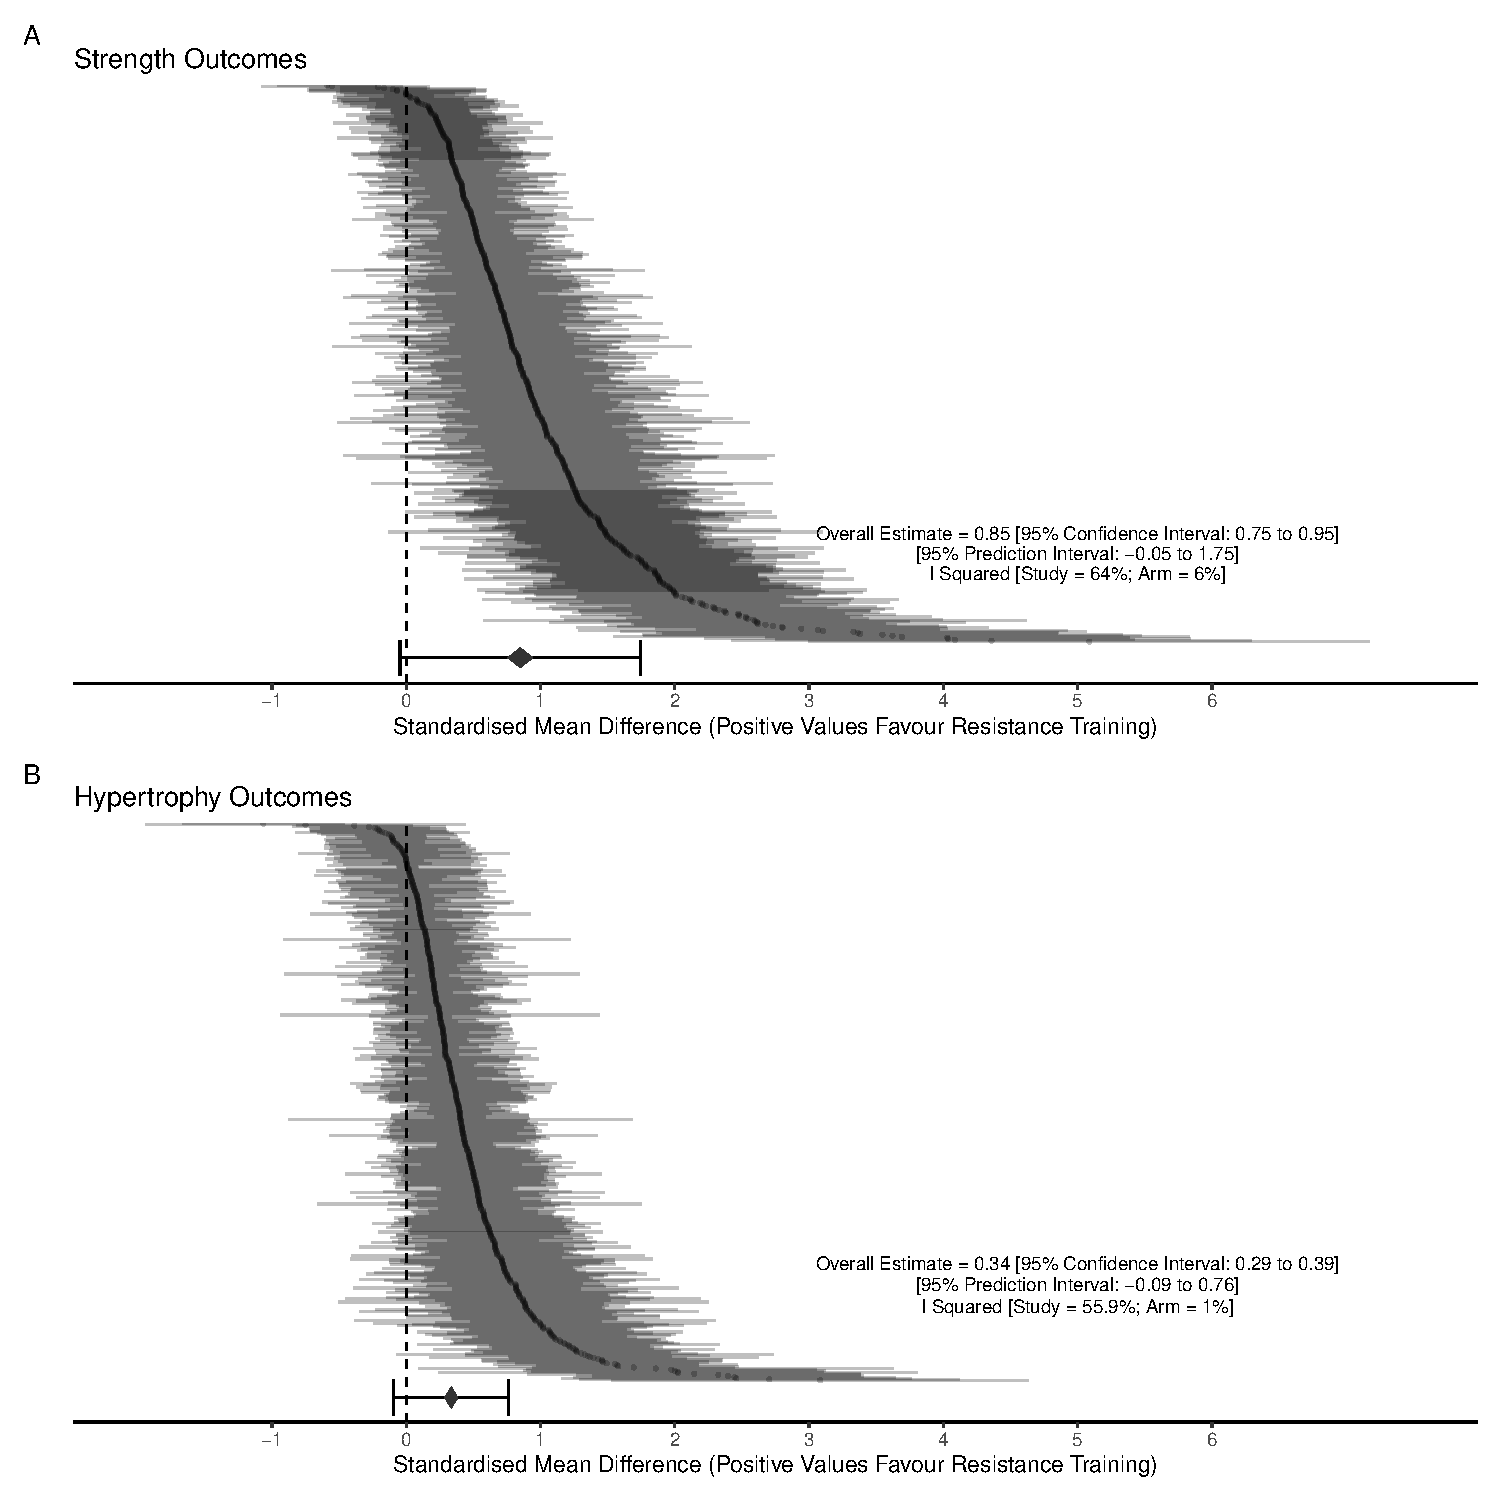
\includegraphics{Revised-Paper---Meta-Analysis-of-Variation-in-Sport-and-Exercise-Science---anonymous_files/figure-latex/forest-SMD-plot-1} 

}

\caption{Caterpillar plots of SMD effect sizes for strength (A) and hypertrophy (B) outcomes.}(\#fig:forest-SMD-plot)
\end{figure}

The pattern of results from our models examining SMDs (figure @ref(fig:forest-SMD-plot)) were similar to those reported by Polito et al. (2021), albeit with slightly lower estimates for both outcome types; possibly due to our use of a multilevel mixed-effects meta-analysis model that allowed for each individual effect size to be more appropriately weighted (the relative amount of heterogeneity between effects for each level is presented as the \(I^2\) statistic). As might be expected, in comparison to non-training controls the RT interventions produced increases in both strength (SMD = 0.87 {[}95\%CI: 0.77 to 0.97{]}; \(I^2_{study}\) = 57.32\%, \(I^2_{arm}\) = 3\%, \(I^2_{effect}\) = 11.95\%) and hypertrophy outcomes (SMD = 0.34 {[}95\%CI: 0.29 to 0.39{]}; \(I^2_{study}\) = 54.62\%, \(I^2_{arm}\) = 0.62\%, \(I^2_{effect}\) = 2.79\%). Confidence intervals on the overall effects were precise for both outcomes though prediction intervals, \textcolor{red}{indicating the range over which we might expect future estimates of effects to fall based on this evidence, for SMD estimates (see figure }@ref(fig:forest-SMD-plot)) \textcolor{red}{were fairly wide and relative heterogeneity was fairly high mostly as a result of between-study variance (i.e., effects were more similar *within* studies and arms than *between* them).}

\begin{figure}

{\centering 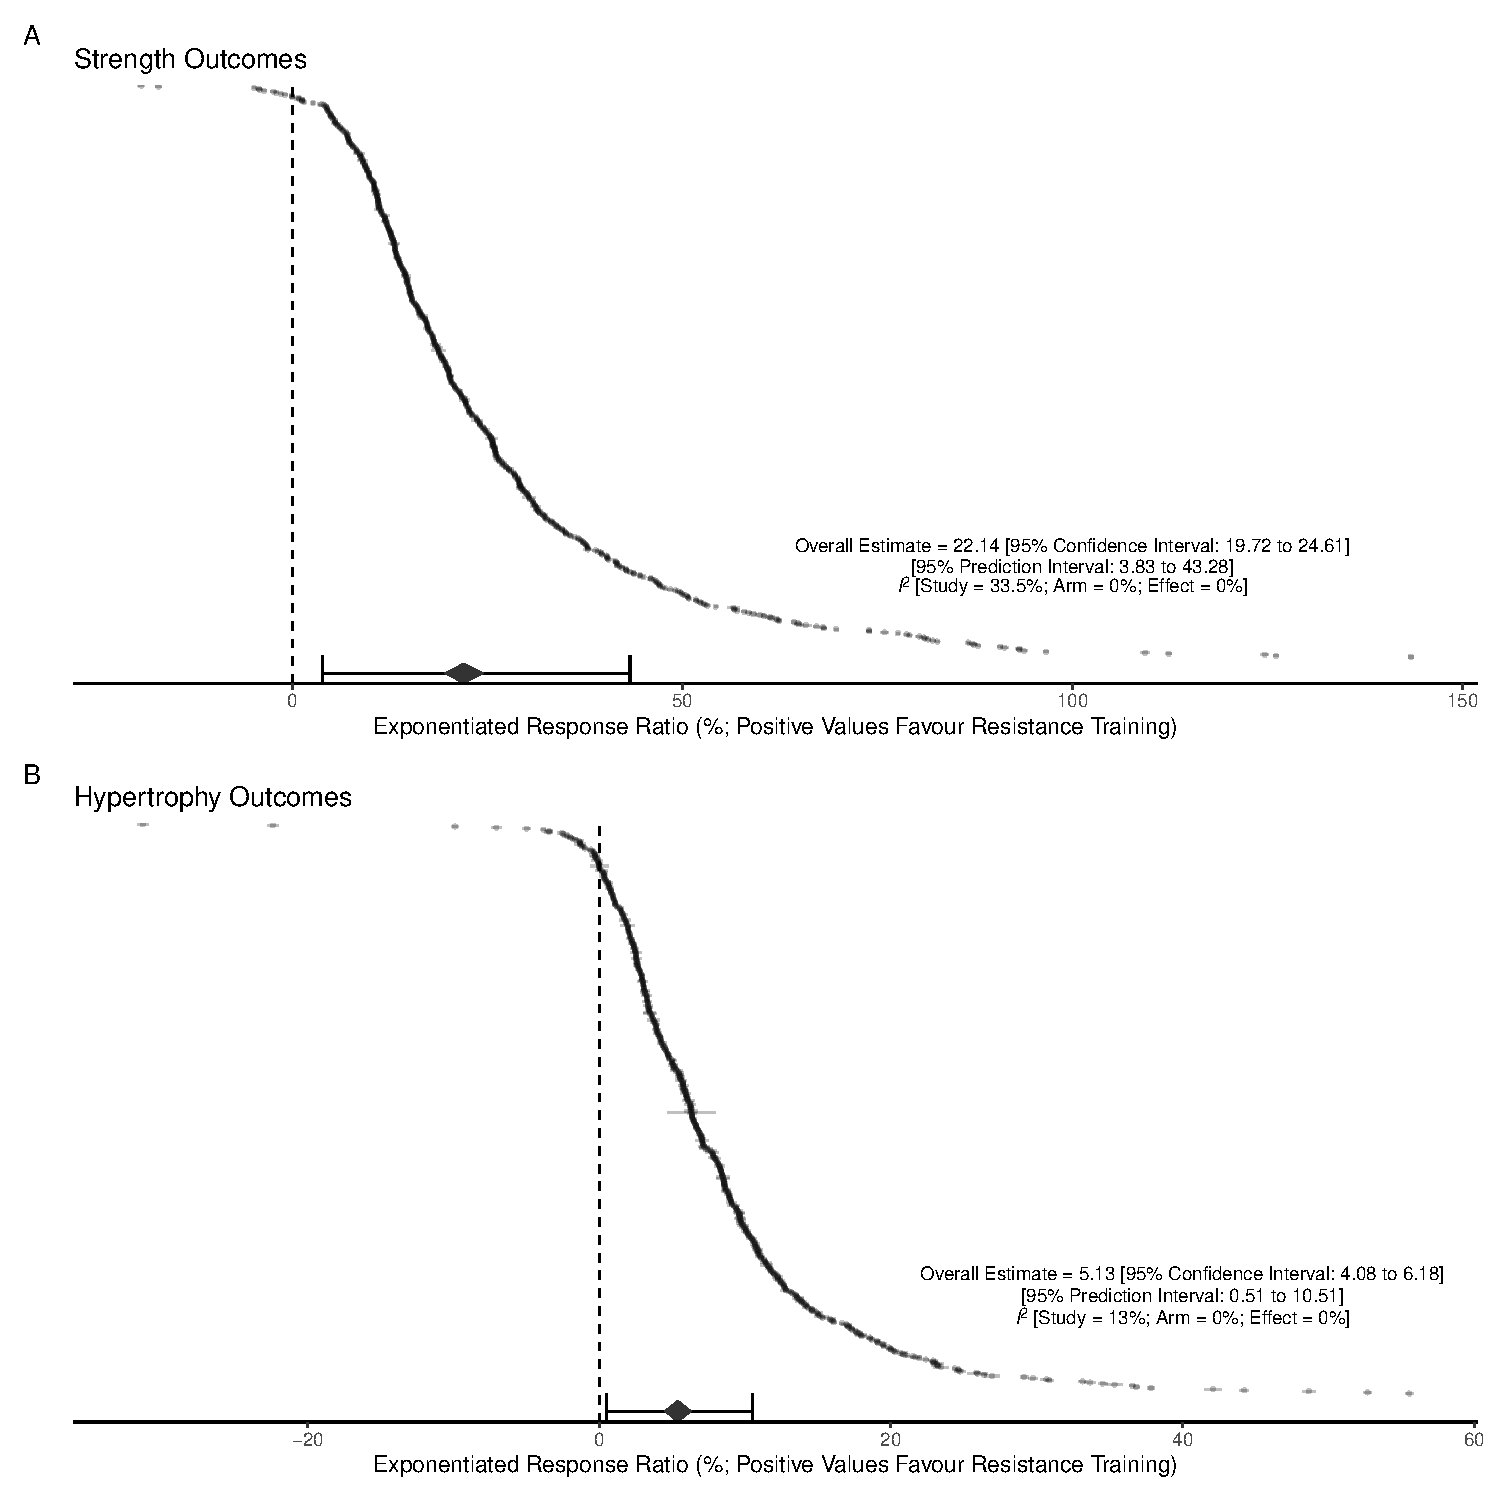
\includegraphics{Revised-Paper---Meta-Analysis-of-Variation-in-Sport-and-Exercise-Science---anonymous_files/figure-latex/forest-RR-plot-1} 

}

\caption{Caterpillar plots of exponentiated RR effect sizes for strength (A) and hypertrophy (B) outcomes.}(\#fig:forest-RR-plot)
\end{figure}

For the \(\textrm{ln}RR\) results we exponentiated them and converted to percentages to be more interpretable. These were similar, with greater proportional increases in strength compared with hypertrophy (figure @ref(fig:forest-RR-plot)). Increases were seen for both strength (\(\textrm{exp}RR\) = 21.97 {[}95\%CI: 19.43 to 24.57{]}; \(I^2_{study}\) = 33.46\%, \(I^2_{arm}\) = 0\%, \(I^2_{effect}\) = 0\%) and hypertrophy (\(\textrm{exp}RR\) = 5.39 {[}95\%CI: 4.44 to 6.35{]}; \(I^2_{study}\) = 12.97\%, \(I^2_{arm}\) = 0\%, \(I^2_{effect}\) = 0\%). Confidence intervals were again precise for both outcomes, and whilst relative heterogeneity was lower compared to SMD models prediction intervals were still quite wide.

In addition to the SMD and \(\textrm{ln}RR\) results, both the \(SD_{ir}\) (figure @ref(fig:forest-SDir-plot)) and \(\textrm{ln}VR\) (figure @ref(fig:forest-logVR-plot)) were also positive for both strength (\(SD_{ir}\) = 0.91 {[}95\%CI: 0.36 to 1.47{]}; \(I^2_{study}\) = 53.85\%, \(I^2_{arm}\) = 0.04\%, \(I^2_{effect}\) = 0\%; \(\textrm{ln}VR\) = 0.9 {[}95\%CI: 0.77 to 1.02{]}; \(I^2_{study}\) = 56.36\%, \(I^2_{arm}\) = 0.77\%, \(I^2_{effect}\) = 27.36\%) and hypertrophy outcomes (\(SD_{ir}\) = 0.42 {[}95\%CI: 0.33 to 0.5{]}; \(I^2_{study}\) = 0.01\%, \(I^2_{arm}\) = 40.15\%, \(I^2_{effect}\) = 39.73\%; \(\textrm{ln}VR\) = 0.5 {[}95\%CI: 0.4 to 0.6{]}; \(I^2_{study}\) = 41.21\%, \(I^2_{arm}\) = 3.31\%, \(I^2_{effect}\) = 33.59\%) indicating that exposure to the RT interventions may have introduced additional variance over and above random error, potentially suggesting the presence of interindividual response variation. Although, heterogeneity across the models and levels (study, arm, effect) were again relatively large and quite varied.

This additional variance might support previous perspectives (Carpinelli, 2017) that the considerable variation in responses to RT interventions typically observed are due to `true' interindividual response variation over and above the random error that occurs from pre- and post-intervention measurements (i.e., the variation is \emph{detectable} independent of the random error). However, as noted, both the \(SD_{ir}\) and \(\textrm{ln}VR\) assume constant variance over values of the mean \textcolor{red}{(i.e., that the variance is similar whether mean values are low or high)}. As we have seen from the SMD and \(\textrm{ln}RR\) models, RT interventions increase mean scores. Thus, if there is a mean-variance relationship in the data, an increase in the mean alone may be fully responsible for any apparent increase in variation. As such, we cannot rely solely on absolute comparisons of variance such as the \(SD_{ir}\) and \(\textrm{ln}VR\) to determine whether interindividual response variation is actually present. The \(\textrm{ln}CVR\) can be used to overcome this issue, and below we re-analyse this dataset using this effect size statistic. First though, we present data demonstrating the ubiquity of the mean-variance relationship in typical RT study outcome measures \textcolor{red}{to emphasise the need to consider this assumption,} and introduce a modelling approach that can also be used to overcome some possible limitations with the \(\textrm{ln}CVR\) \textcolor{red}{and provide flexibility to accomodate wider applications}.

\begin{figure}

{\centering 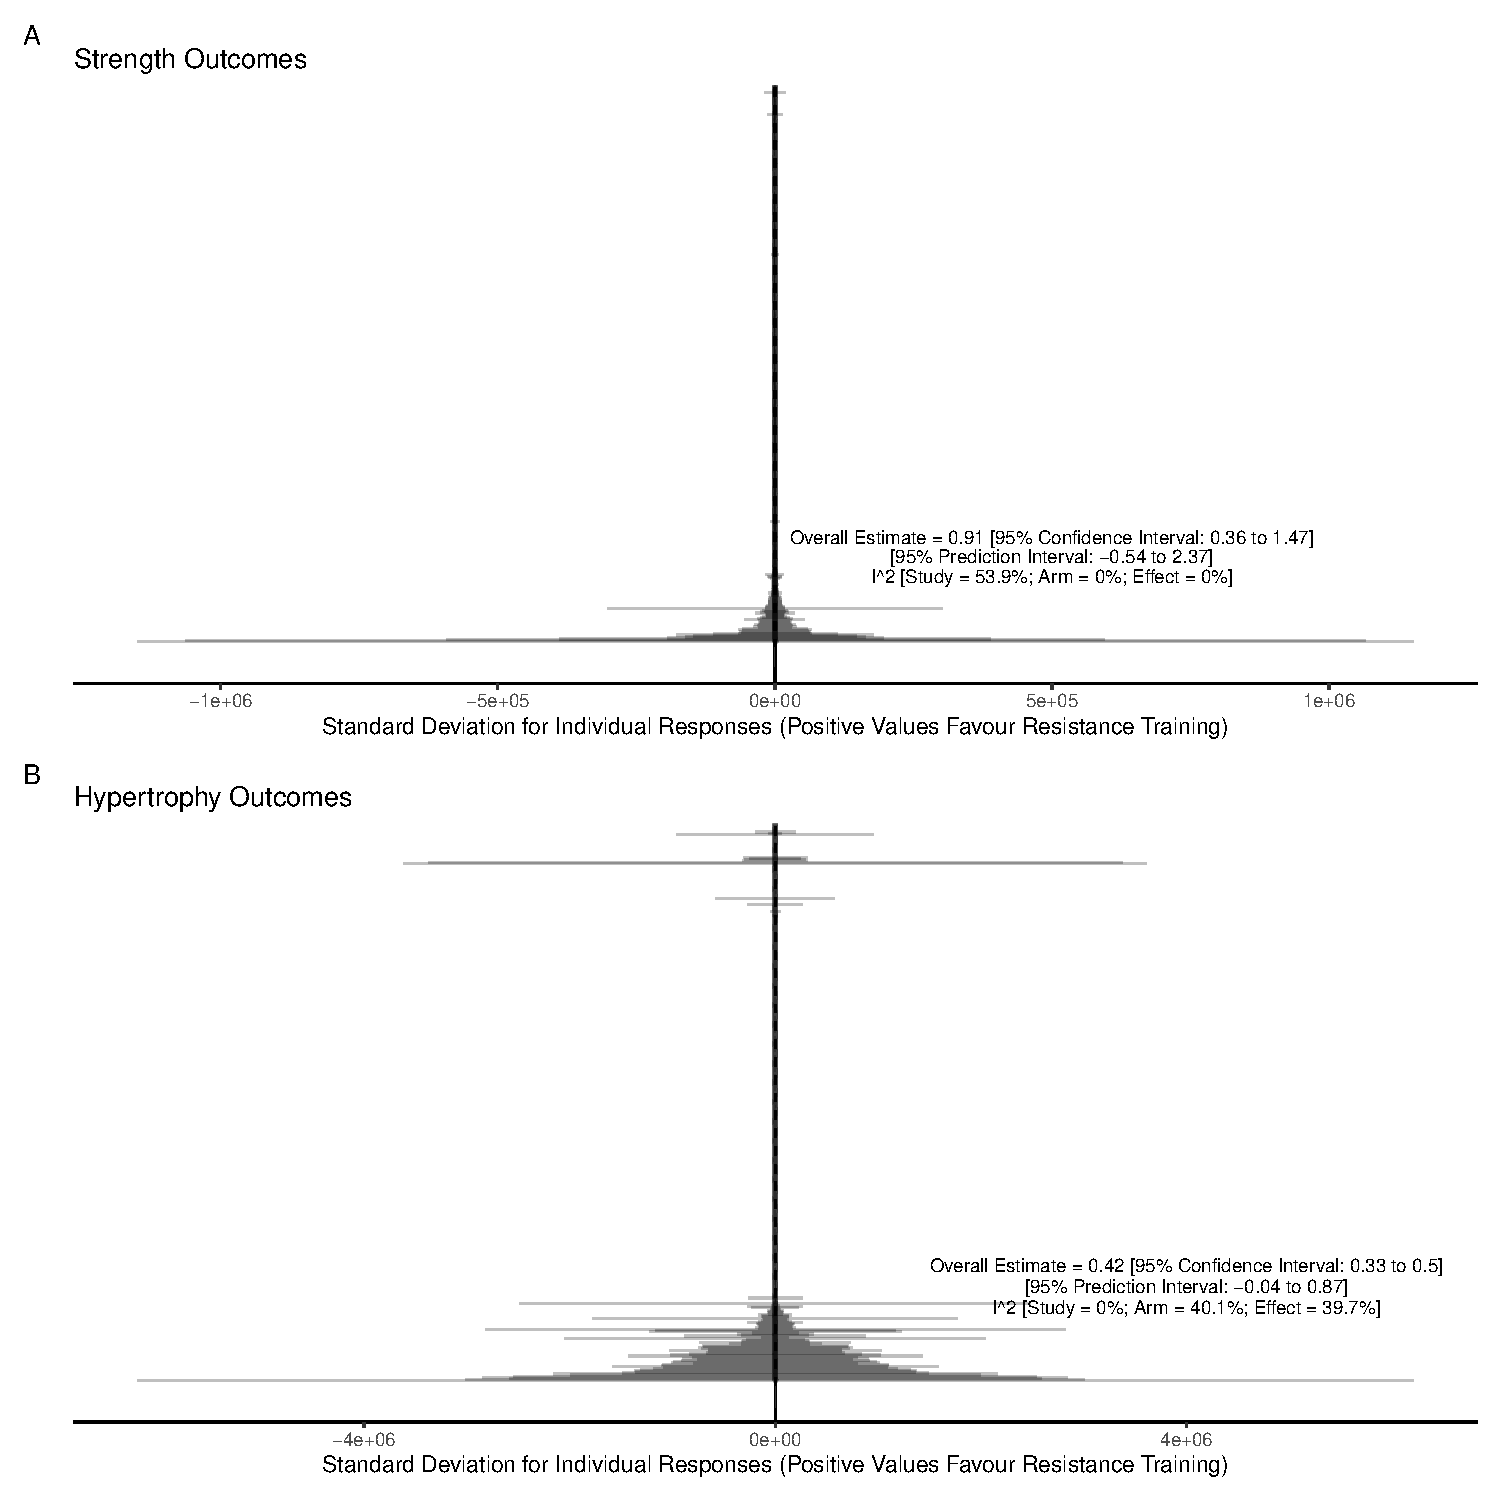
\includegraphics{Revised-Paper---Meta-Analysis-of-Variation-in-Sport-and-Exercise-Science---anonymous_files/figure-latex/forest-SDir-plot-1} 

}

\caption{Caterpillar plots of SDir effect sizes for strength (A) and hypertrophy (B) outcomes.}(\#fig:forest-SDir-plot)
\end{figure}
\begin{figure}

{\centering 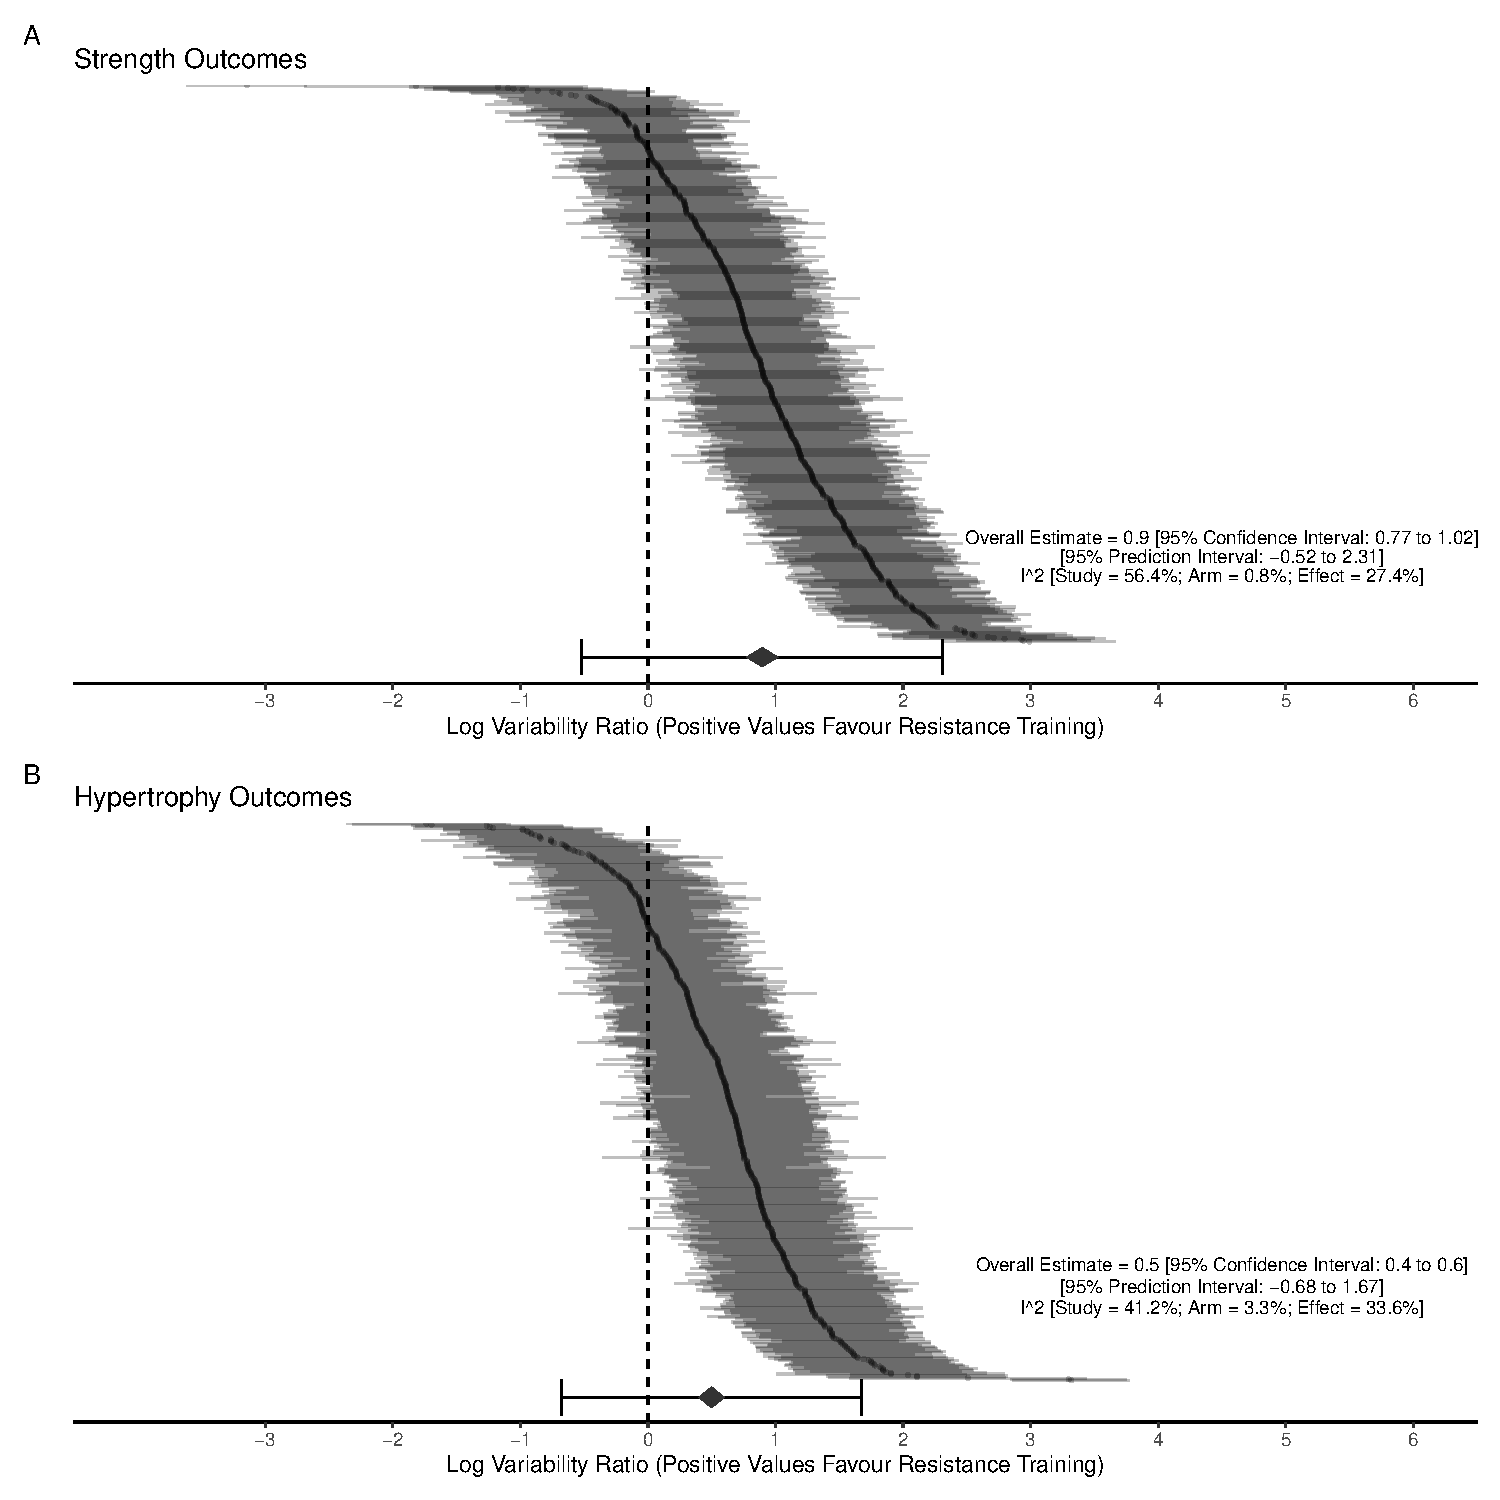
\includegraphics{Revised-Paper---Meta-Analysis-of-Variation-in-Sport-and-Exercise-Science---anonymous_files/figure-latex/forest-logVR-plot-1} 

}

\caption{Caterpillar plots of ln$VR$ effect sizes for strength (A) and hypertrophy (B) outcomes.}(\#fig:forest-logVR-plot)
\end{figure}

\hypertarget{mean-variance-relationships-in-muscular-strength-and-hypertrophy}{%
\subsection{Mean-variance relationships in muscular strength and hypertrophy}\label{mean-variance-relationships-in-muscular-strength-and-hypertrophy}}

With meta-analytic models of variation we are not limited to solely exploring variation in responses to interventions (e.g., Halperin et al. (2022); Nuzzo et al. (2023b)). We can explore the relationships between variance in a number of outcomes and the impact of certain predictors on this in the form of meta-regression. For example, as noted, one possible predictor of variance is the mean itself. As such, we can model variance of each effect as the response itself with the mean of the effect as the predictor. The standard deviation is, however, bounded at zero and so in many cases it may not conform to assumptions of normality which are required for regression models \textcolor{red}{(i.e., that the residuals, the difference between the estimated and actual data, are normally distributed).} Therefore, we instead can use \(\textrm{ln}\hat\sigma\), which is unbounded. In the following example we explore the mean-variance relationship in the pre-intervention scores for outcomes in the data set from Polito et al. (2021).

\begin{figure}

{\centering 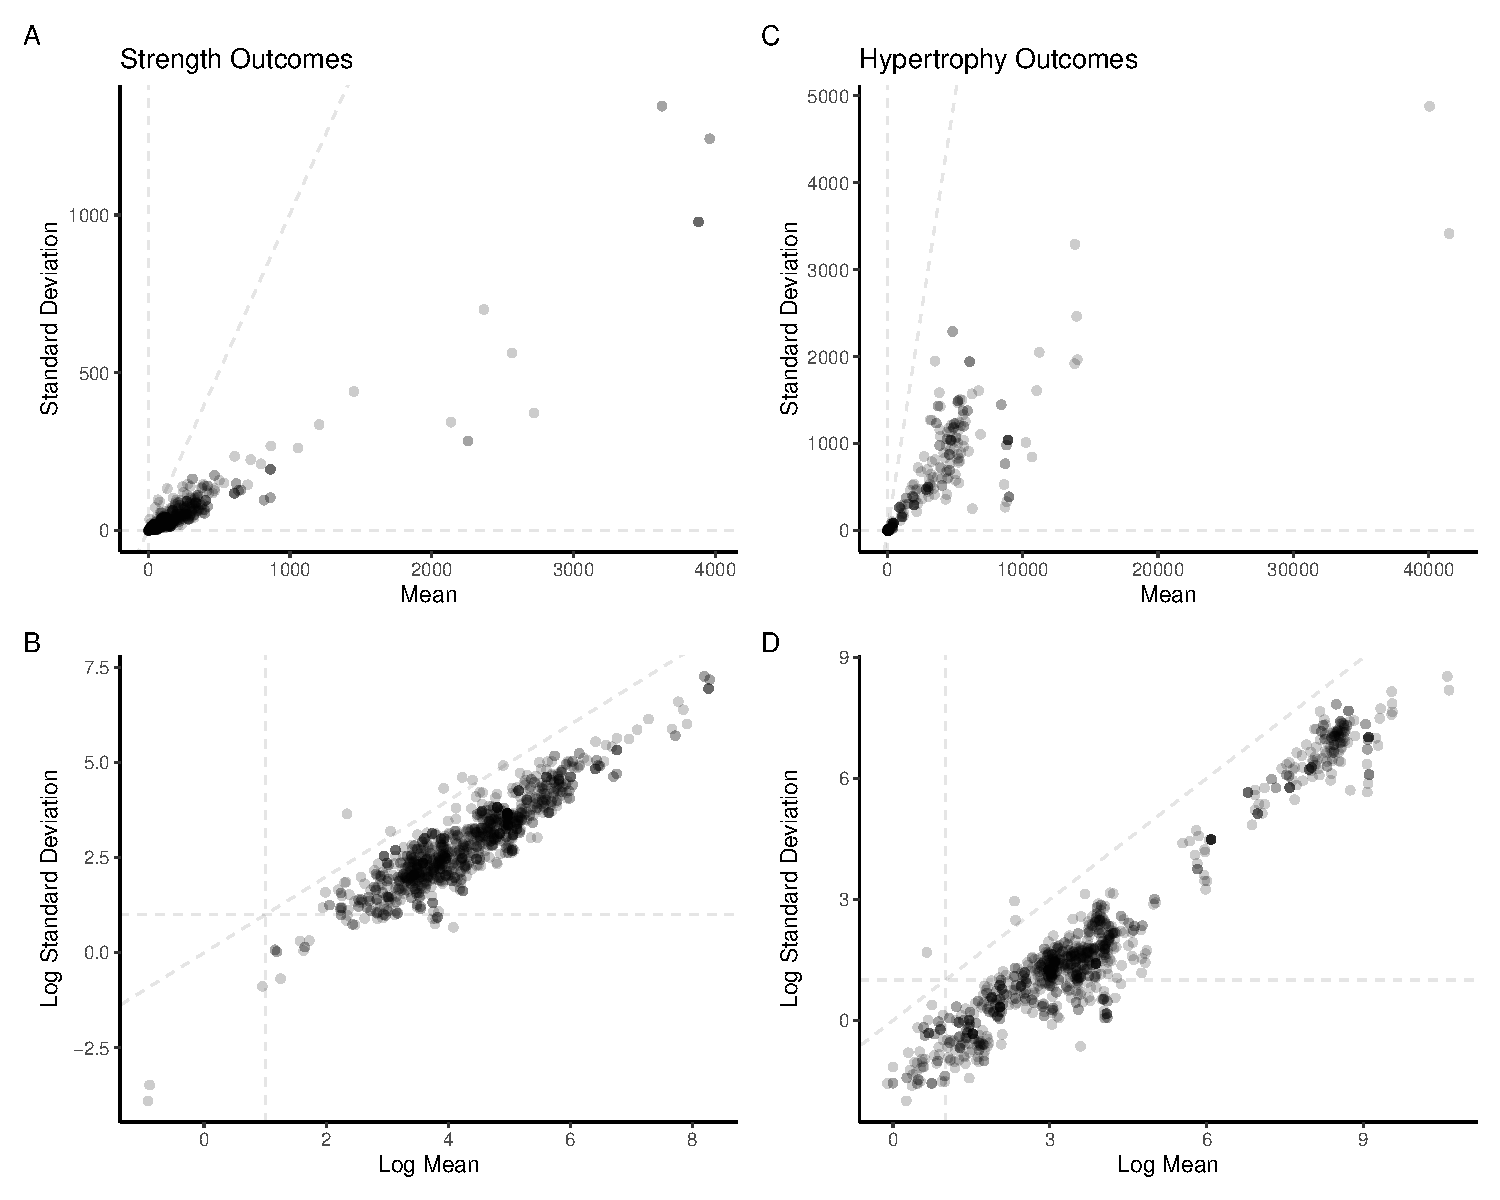
\includegraphics{Revised-Paper---Meta-Analysis-of-Variation-in-Sport-and-Exercise-Science---anonymous_files/figure-latex/mean-variance-pre-plot-1} 

}

\caption{Scatter plots of raw mean and standard deviation of pre-intervention scores for (A) strength outcomes and (B) hypertrophy outcomes, and of the log mean and log standard deviation of pre-intervention scores for (C) strength outcomes and (D) hypertrophy outcomes.}(\#fig:mean-variance-pre-plot)
\end{figure}

As can be seen in figure @ref(fig:mean-variance-pre-plot)(A) and (C), there is considerable heteroskedasticity in the relationship between the raw mean (\(\overline{x}\)) and standard deviation (\(s\)). \textcolor{red}{The variance in standard deviations increases with higher mean values.} This is similar to what is known as Taylor's law in ecology, or the power law; in essence, an empirically derived relationship stating that the variance is a power function of the mean in many biological and physical systems (Taylor, 1961).

\begin{equation}
s^2=a\overline{x}^b
(\#eq:taylors-eq)
\end{equation}

where \(a\) and \(b\) are some constants. When this relationship holds, under most circumstances the standard deviation is not proportional to the mean. However, when the mean and standard deviation are transformed to the log scale this relationship becomes linear \textcolor{red}{based upon the product and power logarithmic rules:}

\begin{equation}
2\textrm{ln}s=\textrm{ln}a+b\textrm{ln}\overline{x}
(\#eq:taylorsln-eq)
\end{equation}

Figure @ref(fig:mean-variance-pre-plot)(B) and (D) shows that the relationship between the mean and variance on the log scale better meets the assumption of normality. Given these the observations we have for \(\textrm{ln}\hat\sigma\) and \(\textrm{ln}\overline{x}\) come from multiple outcomes within multiple arms within studies we can also estimate this relationship using a multilevel mixed-effects meta-regression model similar to that applied above. In this case though we are including an additional \emph{predictor} variable, the \(\textrm{ln}\overline{x}\). For example, the following model specifies \(\textrm{ln}\overline{x}\) as a fixed effect with random intercepts for study, arm, and effect:

\begin{equation}
\textrm{ln}\hat\sigma_{ijk}=(\beta_{0}+\tau_{(1)i}+\tau_{(2)j}+\tau_{(3)k})+\beta_{1}\textrm{ln}\overline{x}_{ijk}+\epsilon_{ijk}+m_{ijk} 
(\#eq:lnm-lns-model-eq)
\end{equation}

where \(\textrm{ln}\hat\sigma_{ijk}\) is the \(k\textrm{th}\) effect size, as in equation @ref(eq:lnsigma-eq), from the \(j\textrm{th}\) arm (\(j = 1,2,\cdots,N_{j}\); where \(N_{j}\) is the number of arms\footnote{In contrast to the models presented examining effect sizes relating to comparisons between and intervention group and control group, in the models examining \(\textrm{ln}\sigma_{ijk}\) and \(\textrm{ln}\overline{x}_{ijk}\) as a predictor the term \emph{arm} refers to both the intervention groups(s) and control group. Thus, where a study had for example two RT interventions and a control, three separate arms would be coded (RT intervention 1, RT intervention 2, and control). Data were again coded such that study and arm had explicit nesting.}) in the \(i\textrm{th}\) study (\(i = 1,2,\cdots,N_{i}\); where \(N_{i}\) is the number of studies), \(\textrm{ln}\overline{x}_{ijk}\) is the mean estimate for each effect size, \(\beta_{0}\) is the intercept or overall mean of the effects, \(\beta_{1}\) is the slope or regression coefficient for \(\textrm{ln}\overline{x}\), \(\tau_{i}\) is the deviation from \(\beta_{0}\) for the \(i\textrm{th}\) study, \(\tau_{j}\) is the deviation for the \(j\textrm{th}\) arm, \(\tau_{k}\) is the deviation for the \(k\textrm{th}\) effect, \(\epsilon_{ijk}\) is the residual for each effect size which is normally distributed with \(\sigma^2_{\epsilon}\), and \(m_{ijk}\) is the sampling error for each effect size normally distributed with \(\sigma^2_{\textrm{ln}\hat\sigma_{ijk}}\).

\textcolor{red}{These kinds of models are highly flexible.} Additional predictor terms could be added; for example, we could model a categorical variable for the outcome type and include \(\beta_{2}Outcome\) in the model with \(Outcome\) as a dummy coded variable for the outcome type (i.e., hypertrophy = 0, and strength = 1), where \(\beta_{2}\) is the slope or regression coefficient for \(Outcome\) (most intuitively thought of as the difference between the two outcome types)\footnote{We do not have to limit ourselves to only fixed effect predictor terms as we have here. Indeed, for mixed effect models generally some argue that models should use a \emph{maximal} random effects structure including both random intercepts and slopes \textcolor{red}{(i.e., that the effect of the predictor term can vary within different levels of the model and is also assumed to come from an overarching distribution of slopes), and their correlations, to enhance generalisability of inferences} (Barr et al., 2013). We could model a categorical variable for the outcome type and using random effects include \((\beta_{2} + \varphi_{i})Outcome\) or \((\beta_{2} + \varphi_{i} + \varphi_{j})Outcome\) in the model with \(Outcome\) as a dummy coded variable for the outcome type (i.e., hypertrophy = 0, and strength = 1), where \(\beta_{2}\) is the overall average slope or regression coefficient for \(Outcome\), and \(\varphi_{i}\) is the deviation (random slope) from \(\beta_{2}\) for the \(i\textrm{th}\) study and \(\varphi_{j}\) is the deviation for the \(j\textrm{th}\) arm. \textcolor{red}{These model specifications do not assume that the difference between outcomes is fixed, but can vary between studies and arms. We could also do the same and include random slopes for $(\beta_{1}$ on $\textrm{ln}\overline{x}$ thus allowing for the strength of the relationship between $\textrm{ln}\hat\sigma$ and $\textrm{ln}\overline{x}$ to also vary between studies and arms. Indeed, we fit a range of models  using $\textrm{ln}\hat\sigma$ with $\textrm{ln}\overline{x}$ and $Outcome$ as a predictor with (1) random intercepts only for study and arm, (2) the inclusion of correlated random slopes for $\textrm{ln}\overline{x}$ by study, (3) the inclusion of correlated random slopes for $\textrm{ln}\overline{x}$ by study and arm, (4) the inclusion of correlated random slopes for $Outcome$ by study, (5) the inclusion of correlated random slopes for $Outcome$ by study and arm, and (6) the inclusion of correlated random slopes for both $\textrm{ln}\overline{x}$ and $Outcome$ by study, (7) the inclusion of correlated random slopes for both $\textrm{ln}\overline{x}$ and $Outcome$ by study and arm.  The comparison of these models using $2\times\textrm{log}BF$} (Kass \& Raftery, 1995) \textcolor{red}{from approximate Bayesian information criterion} (Wagenmakers, 2007) \textcolor{red}{to determine under which is the observed data most likely is included in the supplementary materials (https://osf.io/3tv6x). There was very strong evidence supporting the random intercepts only model compared to all others and so this is presented here.}}.

Figure @ref(fig:model-mean-variance-pre-plot) shows this model fit visually where the size of the points reflects their weight in the model. Both strength and hypertrophy outcomes show strong linearity between the mean and standard deviation on the log scale, though there is a small difference in intercepts between the two outcome types suggesting a slight but systematically greater degree of variance in strength measures compared to hypertrophy for a given mean score.

\begin{figure}

{\centering 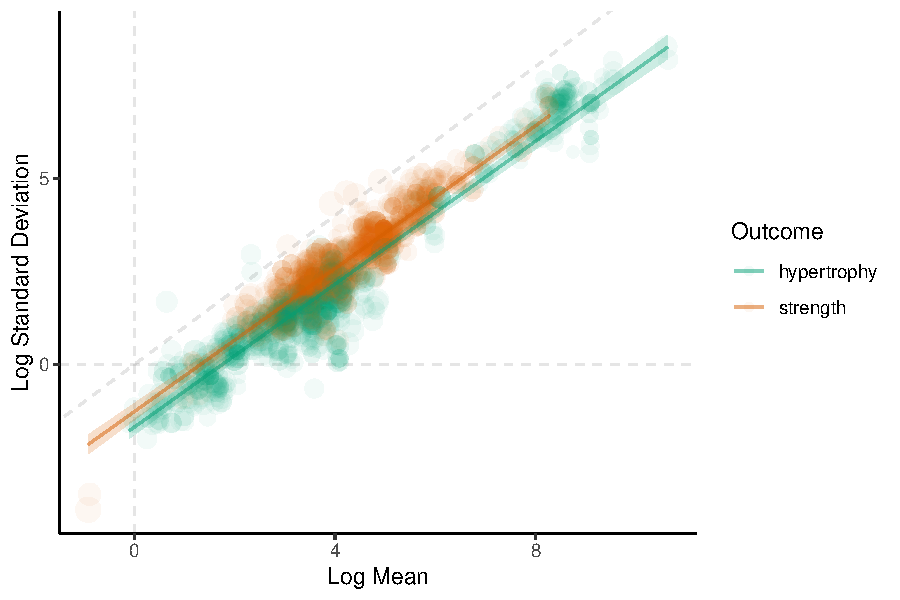
\includegraphics{Revised-Paper---Meta-Analysis-of-Variation-in-Sport-and-Exercise-Science---anonymous_files/figure-latex/model-mean-variance-pre-plot-1} 

}

\caption{Meta-analytic scatter plot of the log mean and log standard deviation of pre-intervention scores.}(\#fig:model-mean-variance-pre-plot)
\end{figure}

The presence of Taylor's law type relationships should be examined in datasets prior to deciding on which variance effect size statistic should be employed. Returning to the context of interindividual response variation to interventions, the presence of a mean-variance relationship in the data would imply that we cannot rely on absolute comparisons of variance (i.e., \(SD_{ir}\) or \(\textrm{ln}VR\)) to determine whether interindividual response variation is actually present. So we should also explore this assumption for the change-scores in the RT and control groups and determining the appropriate effect sizes to explore.

\hypertarget{reanalysis-of-interindividual-response-variation-using-textrmlncvr}{%
\subsection{\texorpdfstring{Reanalysis of interindividual response variation using \(\textrm{ln}CVR\)}{Reanalysis of interindividual response variation using \textbackslash textrm\{ln\}CVR}}\label{reanalysis-of-interindividual-response-variation-using-textrmlncvr}}

As can be seen in figures @ref(fig:mean-variance-delta-plot)(A) and (C) there is also a mean-variance relationship in the change score data about zero whereby an increase in the mean alone (i.e., greater mean change score in the intervention compared to the control) may be fully responsible for any apparent increase in variation. Further, when transforming change scores to absolute changes (i.e., converting all to positive numeric scores) we see that in figures @ref(fig:mean-variance-delta-plot)(B) and (D) that the log transformation exhibits similar linearity as seen with the pre-intervention scores above. As such, in this case, we cannot rely solely on absolute comparisons of variance such as the \(SD_{ir}\) and \(\textrm{ln}VR\) to determine whether interindividual response variation is actually present.

\begin{figure}

{\centering 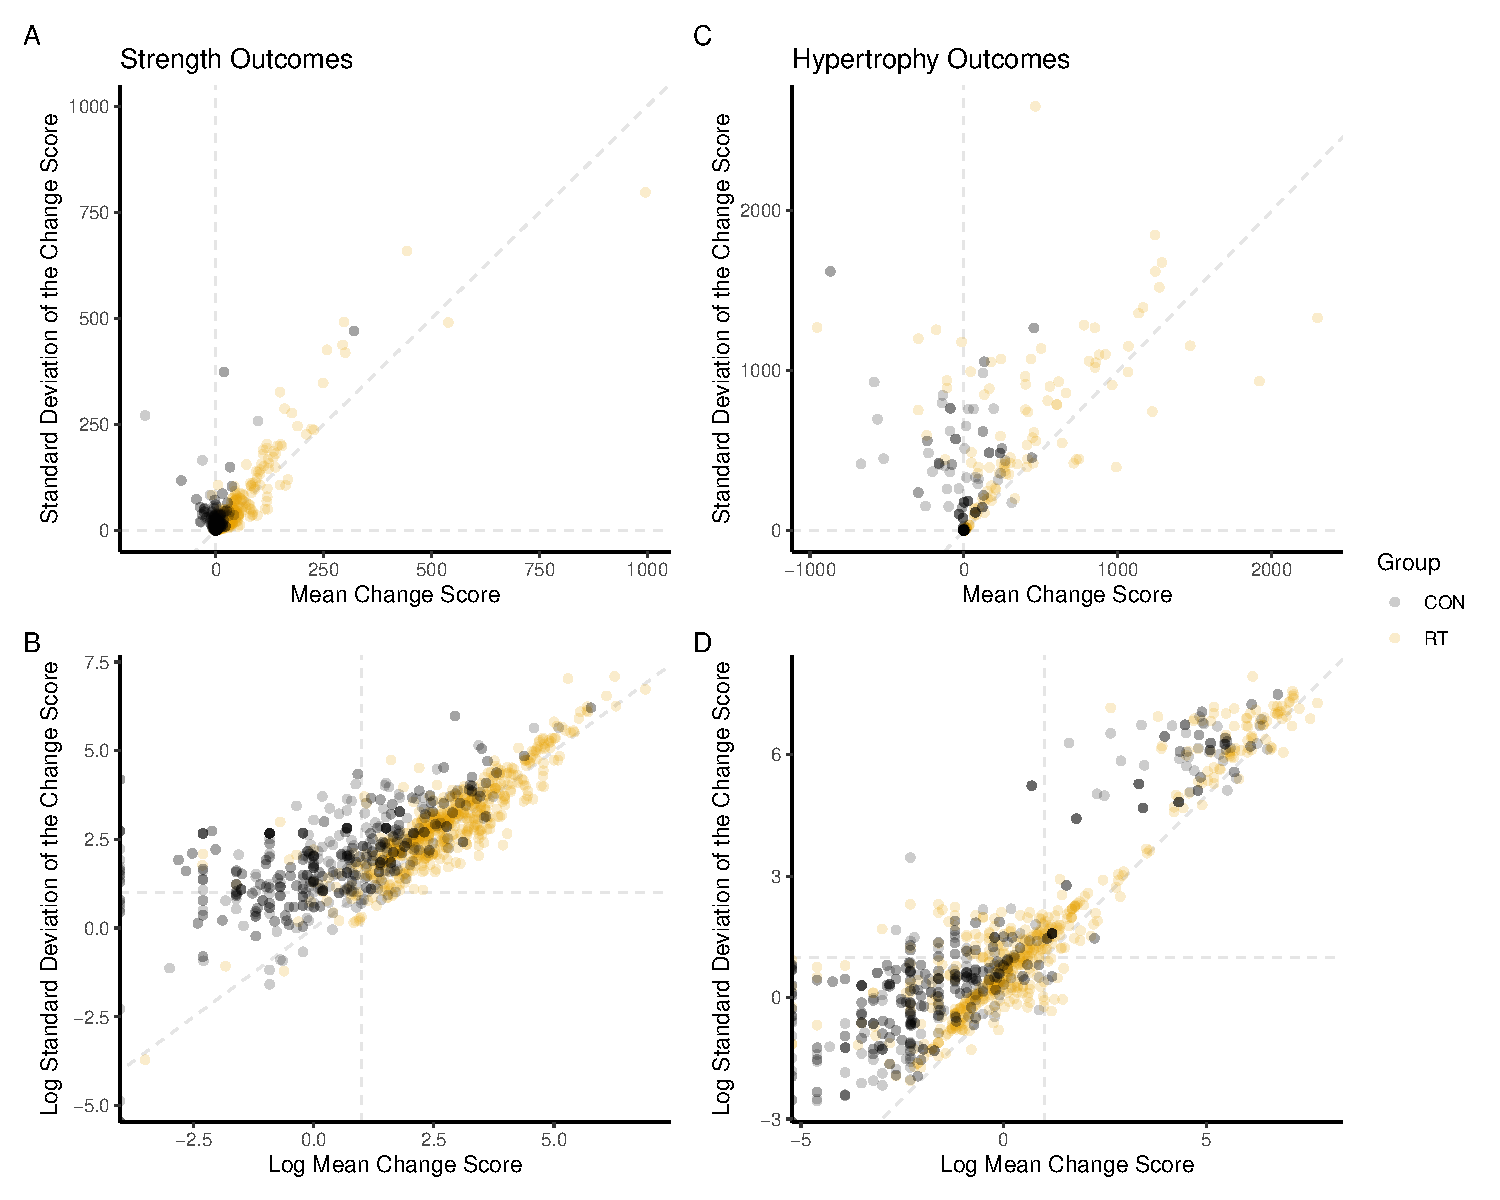
\includegraphics{Revised-Paper---Meta-Analysis-of-Variation-in-Sport-and-Exercise-Science---anonymous_files/figure-latex/mean-variance-delta-plot-1} 

}

\caption{Scatter plots of raw mean and standard deviation of change scores for (A) strength outcomes and (B) hypertrophy outcomes, and of the log mean and log standard deviation of change scores for (C) strength outcomes and (D) hypertrophy outcomes.}(\#fig:mean-variance-delta-plot)
\end{figure}

The \(\textrm{ln}CVR\) can be used to overcome this issue though. Fitting the same multilevel mixed-effects meta-analysis model with cluster-robust variance estimation and random intercepts for study, arm, and effect as before (see equation @ref(eq:ml-model-eq)) using the \(\textrm{ln}CVR\) as the effect size statistic leads to different conclusions compared to absolute variance comparisons using \(SD_{ir}\) or \(\textrm{ln}VR\). The introduction of an RT intervention actually \emph{reduces} the relative variation seen in change scores for strength (\(\textrm{ln}CVR\) = -0.61 {[}95\%CI: -0.76 to -0.47{]}; \(I^2_{study}\) = 23.18\%, \(I^2_{arm}\) = 0\%, \(I^2_{effect}\) = 0\%) and hypertrophy (\(\textrm{ln}CVR\) = -0.45 {[}95\%CI: -0.61 to -0.29{]}; \(I^2_{study}\) = 10.03\%, \(I^2_{arm}\) = 0\%, \(I^2_{effect}\) = 0\%) and further there is lower relative heterogeneity between studies in the effect estimates (figure @ref(fig:forest-logCVR-plot)).

\begin{figure}

{\centering 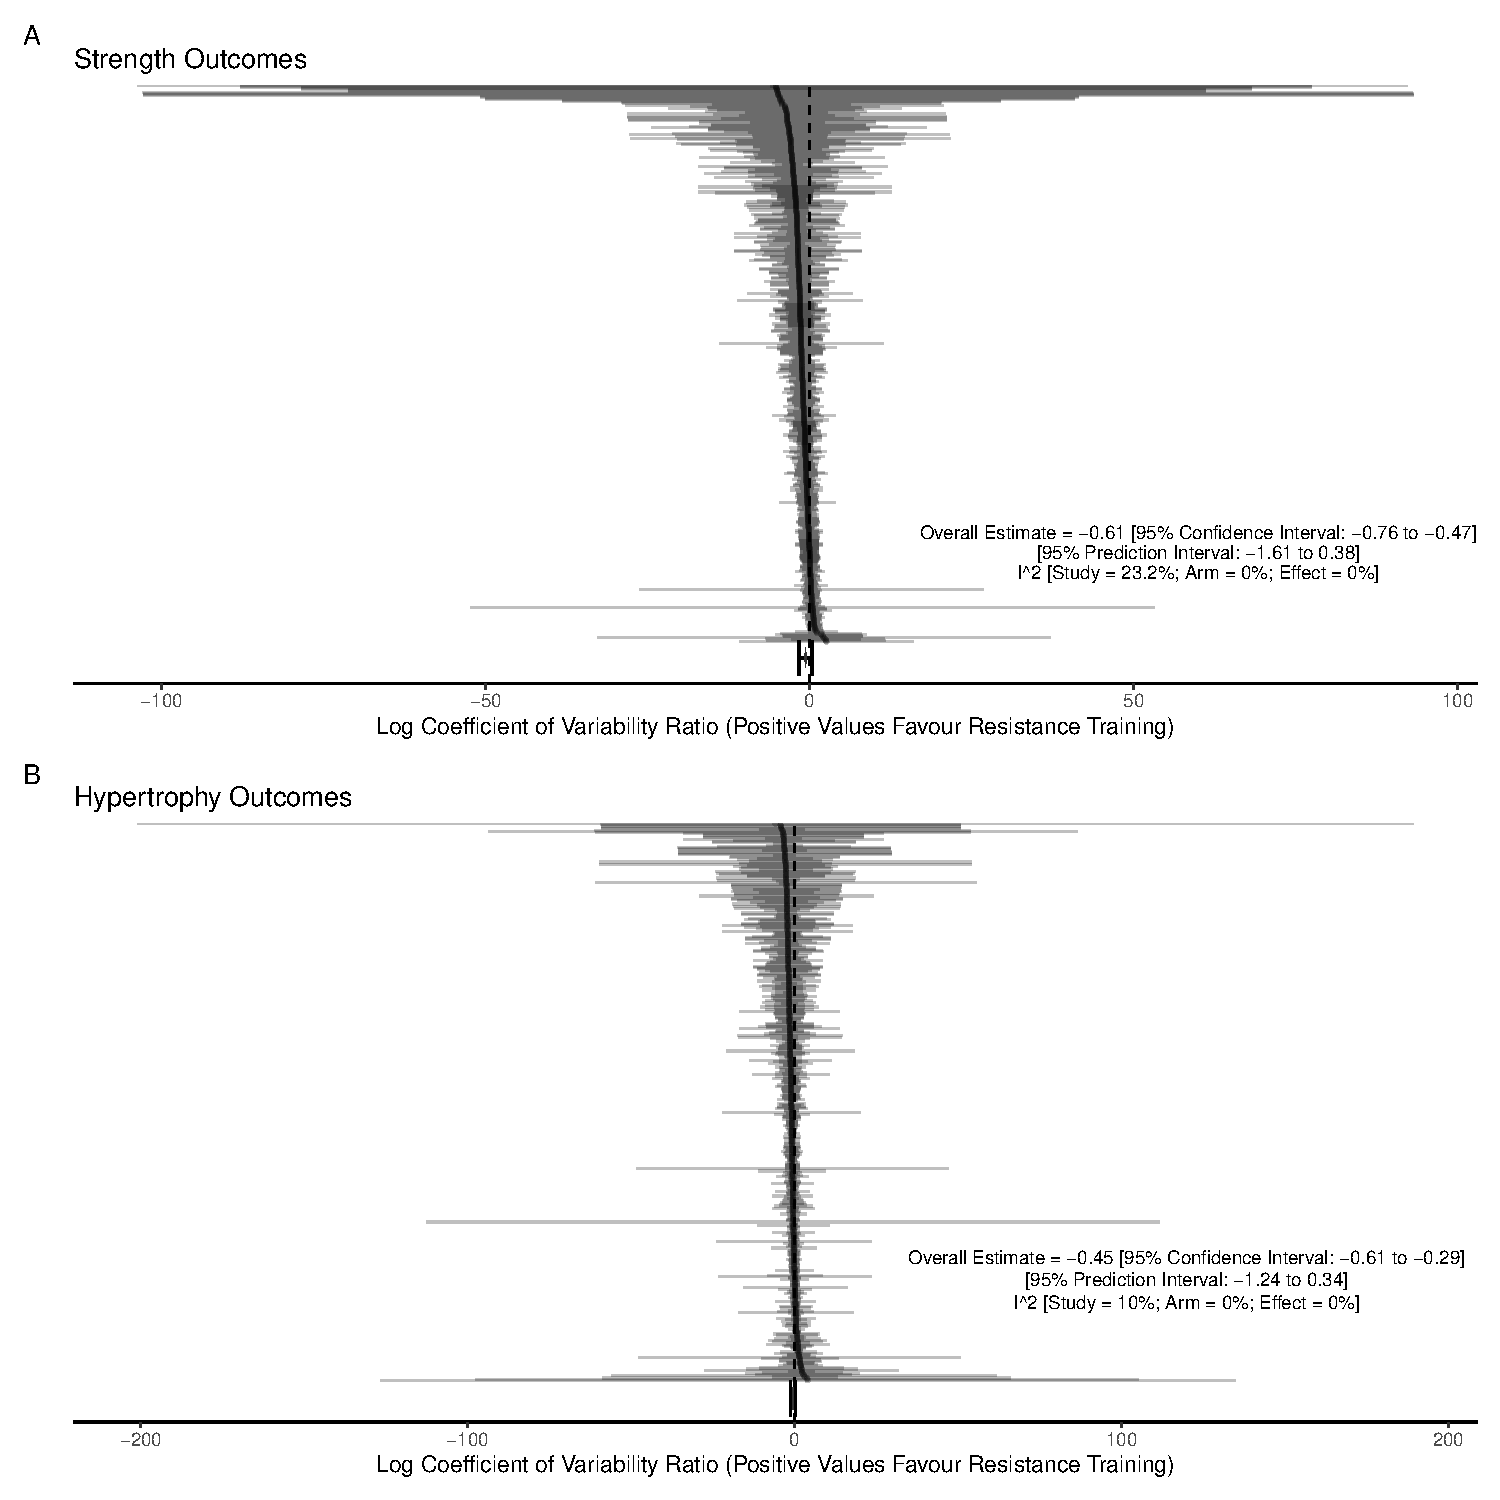
\includegraphics{Revised-Paper---Meta-Analysis-of-Variation-in-Sport-and-Exercise-Science---anonymous_files/figure-latex/forest-logCVR-plot-1} 

}

\caption{Caterpillar plots of ln$CVR$ effect sizes for strength (A) and hypertrophy (B) outcomes.}(\#fig:forest-logCVR-plot)
\end{figure}

There is, however, a potential limitation for the \(\textrm{ln}CVR\) also that may need to be considered. Firstly, it is limited to the use of ratio scale data (which is not the case for the \(\textrm{ln}\hat\sigma\) or \(\textrm{ln}VR\)); hence the need to transform the change scores to be positively signed in this specific case. Secondly, whilst the \(\textrm{ln}CVR\) is useful in situations where there is a mean-variance relationship, the use of the \(CV\) in the effect size statistic assumes proportionality between standard deviation and mean. Where we see the kind of heteroskedasticity in the relationship between mean and standard deviation as we do for the change scores here (figure @ref(fig:mean-variance-delta-plot)) an alternative yet \textcolor{red}{comparable} approach might be desirable. \textcolor{red}{Lastly, this statistic is limited to examination of pairwise comparisons of variance. In this example this approach poses no issue as we are comparing RT intervention group(s) to a control group. But, as seen with the pre-score example above, alternative modelling approaches provide greater flexibility and can still offer estimation of a \textcolor{red}{comparable} effect of interest to the $\textrm{ln}CVR$ one just applied.}

\hypertarget{meta-regression-of-textrmlnhatsigma-with-textrmlnoverlinex-and-group}{%
\subsection{\texorpdfstring{Meta-regression of \(\textrm{ln}\hat\sigma\) with \(\textrm{ln}\overline{x}\) and \(Group\)}{Meta-regression of \textbackslash textrm\{ln\}\textbackslash hat\textbackslash sigma with \textbackslash textrm\{ln\}\textbackslash overline\{x\} and Group}}\label{meta-regression-of-textrmlnhatsigma-with-textrmlnoverlinex-and-group}}

Instead, we can use a version of the meta-regression model described above (see equation @ref(eq:lnm-lns-model-eq) and the paragraph which followed it) to compare the variability in change scores between intervention and control groups using \(\textrm{ln}\hat\sigma\) and \(\textrm{ln}\overline{x}\). In this case, the categorical variable for the outcome type used previously is instead swapped for the group type and the new model term included becomes \(\beta_{2}Group\) with \(Group\) as a dummy coded variable for the group (i.e., non-training control = 0, and RT intervention = 1), where \(\beta_{2}\) is the slope or regression coefficient for \(Group\). \textcolor{red}{This kind of meta-regression model with  $Group$ as a predictor is comparable to the $\textrm{ln}CVR$ model in the previous section where the $\beta_{2}Group$ is the slope or regression coefficient for $Group$ and reflects the difference i.e., variance in the RT groups vs the control groups. This reflects the pairwise nature of the $\textrm{ln}CVR$.}

\begin{figure}

{\centering 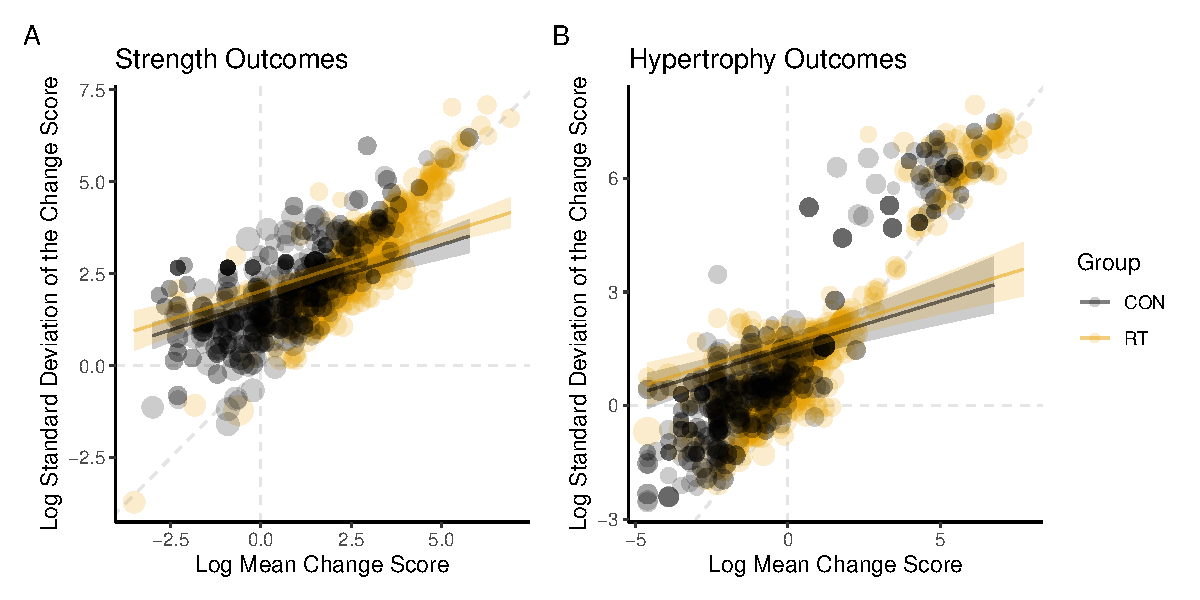
\includegraphics{Revised-Paper---Meta-Analysis-of-Variation-in-Sport-and-Exercise-Science---anonymous_files/figure-latex/model-mean-variance-delta-plot-1} 

}

\caption{Meta-analytic scatter plot of the log mean and log standard deviation of change scores.}(\#fig:model-mean-variance-delta-plot)
\end{figure}

Given the heteroskedasticity in the change scores means and standard deviations (see figure @ref(fig:mean-variance-delta-plot)), we fit this model and other model specifications\footnote{Note, as with the models examining \(Outcome\) upon baseline scores, we similarly explored \(\textrm{ln}\hat\sigma\) with \(\textrm{ln}\overline{x}\) and \(Group\) as a predictor with \textcolor{red}{(1) random intercepts only for study and arm, (2) the inclusion of correlated random slopes for $\textrm{ln}\overline{x}$ by study, (3) the inclusion of correlated random slopes for $\textrm{ln}\overline{x}$ by study and arm, (4) the inclusion of correlated random slopes for $Group$ by study, (5) the inclusion of correlated random slopes for both $\textrm{ln}\overline{x}$ and $Group$ by study, and (6) the inclusion of correlated random slopes for both $\textrm{ln}\overline{x}$ and $Outcome$ by study and $\textrm{ln}\overline{x}$ by arm (we do not include the models with random slopes for $Group$ by arm as in this model each arm refers to a particular group, RT or CON, and so no arm provides data for both).  The comparison of these models using $2\times\textrm{log}BF$} (Kass \& Raftery, 1995) \textcolor{red}{from approximate Bayesian information criterion} (Wagenmakers, 2007) \textcolor{red}{to determine under which is the observed data most likely is included in the supplementary materials (see https://osf.io/b5deh for strength and https://osf.io/5ektd for hypertrophy). Similar to the models including $Outcome$ there was very strong evidence supporting the random intercepts only model compared to all others and so this is presented here. All estimates for the difference between RT and CON, where positive values indicate RT *increased* variation in changes scores and negative values indicate it *decreased* variation, can be seen in the supplementary materials (https://osf.io/5g7ce) all of which revealed similar conclusions.}}\textsuperscript{,}\footnote{\textcolor{red}{It is perhaps worth explaining the assumptions that the different models explored make regarding the mean-variance relationship. For example, the $\textrm{ln}VR$ and $\textrm{ln}CVR$ models can be thought of as similar in that they both make fixed assumptions about the relationship between mean and variance; in the $\textrm{ln}VR$ it is assumed to be zero, and in the $\textrm{ln}CVR$ it is assumed to be proportional i.e., one. In both however this is a *strong* assumption. The multilevel meta-regressions on the other hand actually *estimate* this relationship (i.e., the value of $\beta_{1}$, the slope or regression coefficient for $\textrm{ln}\overline{x}$) and in model where random slopes are included this is also estimated allowing it to vary between studies and arms (i.e., in some studies there may be a more or less strong relationship compared to others). Mean-variance relationships are important to consider when exploring variance effects, but it is also important to consider whether or not this relationship is assumed to be some fixed proportional value (i.e., as the $\textrm{ln}CVR$ does) or whether or not this should be estimated from the data and whether it might also vary across studies and arms (i.e., as the multilevel meta-regression models allow). It should also be noted that these models all assume that the $\overline{x}$ is estimated without error which is clearly not the case. Given that for most effects that might be included in such models we can determine the sampling variance for $\overline{x}$ one approach to address this might be to employ models that incorporate the variance on this predictor (i.e., measurement error or errors in variables models). This is beyond the scope of this paper to discuss. It is not necessarily clear which model should be preferred here, and fortunately substantive conclusions are impacted little by model specification, but thought should be given to the assumptions each makes and the fit of each model to the data.}} to the dataset (see figure @ref(fig:model-mean-variance-delta-plot)). The results were largely similar to those found using the \(\textrm{ln}CVR\) model for strength (\(\beta_{\textrm{ln}\hat\sigma[Group \textrm{ for RT}]}\) = -0.34 {[}95\%CI: -0.54 to -0.13{]}) and hypertrophy (\(\beta_{\textrm{ln}\hat\sigma[Group \textrm{ for RT}]}\) = -0.47 {[}95\%CI: -0.71 to -0.22{]}). Both models suggest that the introduction of the RT interventions \emph{reduced} variance in change scores.

\hypertarget{moderators-of-variance-effects}{%
\subsection{Moderators of variance effects}\label{moderators-of-variance-effects}}

\textcolor{red}{Hopefully it is clear from the meta-regression models here, where we have included both fixed and random predictors as both categorical (i.e., $Outcome$, or $Group$) and continuous (i.e., $\textrm{ln}\overline{x}$) variables, that there is considerable flexibility in the inclusion of predictors when exploring variance through a meta-analytic framework. Of course, the pairwise models described can also be extended to meta-regressions to explore not only how study, arm, or effect level characteristics moderate effect size estimates when considering effect sizes such as SMDs or $\textrm{ln}RR$, but also when considering the variance-based effect size statistics and models employed in this article (i.e., $SD_{ir}$, $\textrm{ln}VR$, $\textrm{ln}CVR$, and $\textrm{ln}\hat\sigma$)}\footnote{See supplementary materials (\url{https://osf.io/e6vpr}) for examples from model estimates for both SMD and \(\textrm{ln}CVR\), (used for simplicity of presenting moderator analysis results) across a range of categorical and continuous predictors for both strength and hypertrophy outcomes. There were no obvious moderators of \(\textrm{ln}CVR\) in particular.}. \textcolor{red}{But these are limited to the pairwise comparisons of a categorical variable as the effect size. The meta-regression models presented here for $\textrm{ln}\hat\sigma$ allow for comparisons to be extended beyond two categories (e.g., intervention, placebo, and control) including any number of arbitrary predictors, fixed and random and assumptions about their correlations.}

\hypertarget{discussion}{%
\section{Discussion}\label{discussion}}

Given the apparent lack of awareness of the utility of meta-analytic frameworks for exploring variance, and the potential value such analyses can offer for the sport and exercise sciences, we have presented some existing effect size statistics and models pertinent to this topic that hopefully will encourage and support researchers in the field to embrace more than just the mean when engaging in quantitative evidence synthesis. Indeed, for a field such as sport and exercise science where sample sizes are typically small, meta-analysis becomes even more valuable as such small samples in primary studies have even lower statistical power to detect differences in variation as compared to means\footnote{Indeed, it can be seen from figures @ref(fig:forest-SDir-plot), @ref(fig:forest-logVR-plot), and @ref(fig:forest-logCVR-plot) that many of the individual study effect estimates have very large sampling errors.} (Yang et al., 2022).

It is of particular interest to note the different conclusions drawn here are dependent on the approach taken to determine from non-training control and RT intervention data whether or not there is \emph{detectable} inter-individual response variation present. \textcolor{red}{We deliberately presented these varying approaches to highlight their assumptions and to aid in readers understanding of their applications. Given the different conclusions drawn from the examples provided, we recommend that researchers consider whether assumptions of simpler approaches are met, or indeed seem reasonable, before their application in specific situations. Where for example there is not an obvious mean-variance relationship it may be appropriate to utilise the $SD_{ir}$ or $\textrm{ln}VR$. However, when this is present in the data then the $\textrm{ln}CVR$ or meta-regression of $\textrm{ln}\hat\sigma$ upon $\textrm{ln}\overline{x}$ may be more appropriate, though assumptions regarding whether this relationship is proportional and fixed should also be considered. The structure of the data also impacts the specific modelling approach to be employed and whether or not assumptions that the mean-variance relationship varies within study or arm levels can be incorporated. Further, depending on the exact research questions it is worth considering balancing model complexity with its ability to provide an answer. If a simple pairwise comparison across a categorical variable is of interest then this can be explored with comparable models using the $\textrm{ln}CVR$ or meta-regression of $\textrm{ln}\hat\sigma$ upon $\textrm{ln}\overline{x}$. But where more complicated predictors, including categories extending beyond just two, are of interest then the flexibility of the latter is desirable to explore. Lastly, it is possible that substantive conclusions might be sensitive to the exact model specifications used. As such, it is worth considering the use of so called *multiverse* approaches to exploring questions such as those pertaining to variation with meta-analysis. With multiverse approaches, instead of having to choose one modelling approach, researchers use the many possible approaches (such as presented here) and explore how sensitive their substantive conclusions might be to nuances of model specifications and assumptions} (Olsson-Collentine et al., 2023; Steegen et al., 2016).

The examples presented herein used data from RT studies included in a recent meta-analysis published in the \emph{Journal of Sport Sciences} (Polito et al., 2021), which hopefully makes them more relatable for researchers in sport and exercise sciences. Examining this data using absolute comparisons of variance such as \(SD_{ir}\) and \(\textrm{ln}VR\) gave the impression that the introduction of the RT intervention likely \emph{increased} variance above random error, suggesting the presence of inter-individual response variation. In the case of RT interventions there is evidently an average intervention effect for strength and hypertrophy which is positive (as seen in the SMD and \(\textrm{ln}RR\) models), yet combined with the results from \(SD_{ir}\) and \(\textrm{ln}VR\) we might conclude that while all likely benefit, some benefit more so than others. Indeed, even if for an intervention there was not clear evidence for average intervention effects, exploring variation in their absence might still be important as interventions with large enough variance could imply that the intervention is at least beneficial to some (Usui et al., 2021). Such results might lead researchers to consider that further research exploring subgroup- or participant-by-intervention interactions is required to maximise successful practical application of such an intervention to avoid negative effects for some, and ensure positive effects for others.

However, similar to the cross-sectional pre-intervention score models reported here (and indeed most physical and biological variables), change scores also demonstrated a mean-variance relationship in addition to heteroskedasticity. The likely more appropriate analyses in this case using the \(\textrm{ln}CVR\) or meta-regression of \(\textrm{ln}\hat\sigma\) upon \(\textrm{ln}\overline{x}\) revealed conclusions in the opposite substantive direction of the absolute variance comparisons; essentially, that the introduction of the RT intervention may have slightly \emph{decreased} change score variance, implying that there is likely little to no interindividual response variation to explain. Interventions, such as RT interventions explored here, which induce both meaningful average treatment effects and also show little evidence suggestive of interindividual variation, are likely to be widely generalisable and so from a practical perspective might offer considerable value in that we can have high expectations that everyone receiving them will likely improve (Usui et al., 2021); that is to say we can assume a constant effect and that the average intervention effect is indicative of the individual intervention effect (Cortés Martínez, 2021). Interventions such as these are valuable for the simplification of guidelines and recommendations. For example, muscle strengthening interventions such as RT are recommended for \emph{everyone} in current physical activity guidelines and in such applications there is likely value in a simple approach to such recommendations (Steele et al., 2017, 2022).

The reason for the apparent reduction in variation after introduction of an RT intervention observed here is not necessarily discernible from this analysis. Perhaps the introduction of an RT intervention has indirect effects that reduce other sources of random variance (e.g., diet, other physical activity etc.; Halliday et al. (2017)), or a ceiling effect on change (i.e., plateau in response; Steele et al. (2022)) has a constraining effect (Cortés Martínez, 2021). However, this potentially represents another interesting area of future study regarding variation; specifically, how to produce interventions that actually reduce variance in an outcome. In other contexts such as sporting performance, interventions to not only positively affect mean performance but also those that reduce variation in performance would be highly desirable.

\hypertarget{conclusion}{%
\section{Conclusion}\label{conclusion}}

Embracing variability and focusing on more than merely the mean differences between groups or conditions, such as intervention and control comparisons, has the potential to inform experimental design and lead to changes in both the approach and direction of follow-up studies. Whether there is evidence of meaningful average intervention effects or not, where considerable variance effects are present it suggests that a meaningful line of research would be to aim at identifying subgroup- or participant-by-intervention interactions using appropriate study designs (Hecksteden et al., 2015). Where variance effects are limited this instead suggests that translational work towards generalisable implementation might be the most meaningful line of future research. Finally, there may be cases where it is in fact desirable to identify interventions that actually reduce variance; for example, improvements in methodological approaches to enhance research (Usui et al., 2021), or interventions to reduce variation in sport performances. Thus, researchers in sport and exercise science should consider exploring variance more systematically, and indeed utilise the meta-analytic framework to support this. This could include the re-analysis of past meta-analyses as we have done here, and indeed researchers conducting future meta-analyses in the field of sport and exercise science should consider the value of concomitantly exploring means and variances utilising the established approaches (Atkinson et al., 2019; Atkinson \& Batterham, 2015; Hopkins, 2015; Mills et al., 2021; Nakagawa et al., 2015; Usui et al., 2021) presented here and echoing the efforts of other recent work (Bonafiglia et al., 2022; Esteves et al., 2021; Fisher et al., 2022; Kelley et al., 2020, 2022; Steele et al., 2021). \textcolor{red}{Researchers should be aware though that the meta-analytic modelling of variance, or indeed any effect size statistics, requires careful consideration of the research question and assumptions that different models make. Substantive conclusions may be sensitive to subtle differences in the approaches we have presented.}

\hypertarget{references}{%
\section{References}\label{references}}

\hypertarget{refs}{}
\begin{CSLReferences}{1}{0}
\leavevmode\vadjust pre{\hypertarget{ref-atkinsonTrueFalseInterindividual2015}{}}%
Atkinson, G., \& Batterham, A. M. (2015). True and false interindividual differences in the physiological response to an intervention. \emph{Experimental Physiology}, \emph{100}(6), 577--588. \url{https://doi.org/10.1113/EP085070}

\leavevmode\vadjust pre{\hypertarget{ref-atkinsonIssuesDeterminationResponders2019}{}}%
Atkinson, G., Williamson, P., \& Batterham, A. M. (2019). Issues in the determination of 'responders' and 'non-responders' in physiological research. \emph{Experimental Physiology}, \emph{104}(8), 1215--1225. \url{https://doi.org/10.1113/EP087712}

\leavevmode\vadjust pre{\hypertarget{ref-barrRandomEffectsStructure2013}{}}%
Barr, D. J., Levy, R., Scheepers, C., \& Tily, H. J. (2013). Random effects structure for confirmatory hypothesis testing: {Keep} it maximal. \emph{Journal of Memory and Language}, \emph{68}(3), 10.1016/j.jml.2012.11.001. \url{https://doi.org/10.1016/j.jml.2012.11.001}

\leavevmode\vadjust pre{\hypertarget{ref-bernardez-vazquezResistanceTrainingVariables2022}{}}%
Bernárdez-Vázquez, R., Raya-González, J., Castillo, D., \& Beato, M. (2022). Resistance {Training} {Variables} for {Optimization} of {Muscle} {Hypertrophy}: {An} {Umbrella} {Review}. \emph{Frontiers in Sports and Active Living}, \emph{4}. \url{https://www.frontiersin.org/articles/10.3389/fspor.2022.949021}

\leavevmode\vadjust pre{\hypertarget{ref-bonafigliaInterindividualDifferencesTrainability2022}{}}%
Bonafiglia, J. T., Swinton, P. A., Ross, R., Johannsen, N. M., Martin, C. K., Church, T. S., Slentz, C. A., Ross, L. M., Kraus, W. E., Walsh, J. J., Kenny, G. P., Goldfield, G. S., Prud'homme, D., Sigal, R. J., Earnest, C. P., \& Gurd, B. J. (2022). Interindividual {Differences} in {Trainability} and {Moderators} of {Cardiorespiratory} {Fitness}, {Waist} {Circumference}, and {Body} {Mass} {Responses}: {A} {Large}-{Scale} {Individual} {Participant} {Data} {Meta}-analysis. \emph{Sports Medicine (Auckland, N.Z.)}. \url{https://doi.org/10.1007/s40279-022-01725-9}

\leavevmode\vadjust pre{\hypertarget{ref-borensteinBasicIntroductionFixedeffect2010}{}}%
Borenstein, M., Hedges, L. V., Higgins, J. P. T., \& Rothstein, H. R. (2010). A basic introduction to fixed-effect and random-effects models for meta-analysis. \emph{Research Synthesis Methods}, \emph{1}(2), 97--111. \url{https://doi.org/10.1002/jrsm.12}

\leavevmode\vadjust pre{\hypertarget{ref-borensteinIntroductionMetaAnalysis2021}{}}%
Borenstein, M., Hedges, L. V., Higgins, J. P. T., \& Rothstein, H. R. (2021). \emph{Introduction to {Meta}-{Analysis}}. John Wiley \& Sons.

\leavevmode\vadjust pre{\hypertarget{ref-caldwellCaseDefaultEffect2020}{}}%
Caldwell, A., \& Vigotsky, A. D. (2020). A case against default effect sizes in sport and exercise science. \emph{PeerJ}, \emph{8}, e10314. \url{https://doi.org/10.7717/peerj.10314}

\leavevmode\vadjust pre{\hypertarget{ref-carpinelliInterindividualHeterogeneityAdaptations2017}{}}%
Carpinelli, R. N. (2017). Interindividual heterogeneity of adaptations to resistance training. \emph{Medicina Sportiva Practica}, \emph{18}(4), 79--94.

\leavevmode\vadjust pre{\hypertarget{ref-cohenStatisticalPowerAnalysis1988}{}}%
Cohen, J. (1988). \emph{Statistical {Power} {Analysis} for the {Behavioral} {Sciences}} (2nd ed.). Routledge. \url{https://doi.org/10.4324/9780203771587}

\leavevmode\vadjust pre{\hypertarget{ref-cortesmartinezConstantEffectRandomized2021}{}}%
Cortés Martínez, J. (2021). Constant effect in randomized clinical trials with quantitative outcome : A methodological review. \emph{TDX (Tesis Doctorals En Xarxa)}. \url{https://upcommons.upc.edu/handle/2117/349575}

\leavevmode\vadjust pre{\hypertarget{ref-curtisMetaanalysisElevatedCO21998}{}}%
Curtis, P. S., \& Wang, X. (1998). A meta-analysis of elevated {CO2} effects on woody plant mass, form, and physiology. \emph{Oecologia}, \emph{113}(3), 299--313. \url{https://doi.org/10.1007/s004420050381}

\leavevmode\vadjust pre{\hypertarget{ref-debQuantifyingEffectsAcute2018}{}}%
Deb, S. K., Brown, D. R., Gough, L. A., Mclellan, C. P., Swinton, P. A., Andy Sparks, S., \& Mcnaughton, L. R. (2018). Quantifying the effects of acute hypoxic exposure on exercise performance and capacity: {A} systematic review and meta-regression. \emph{European Journal of Sport Science}, \emph{18}(2), 243--256. \url{https://doi.org/10.1080/17461391.2017.1410233}

\leavevmode\vadjust pre{\hypertarget{ref-estevesIndividualParticipantData2021}{}}%
Esteves, G. P., Swinton, P., Sale, C., James, R. M., Artioli, G. G., Roschel, H., Gualano, B., Saunders, B., \& Dolan, E. (2021). Individual {Participant} {Data} {Meta}-{Analysis} {Provides} {No} {Evidence} of {Intervention} {Response} {Variation} in {Individuals} {Supplementing} {With} {Beta}-{Alanine}. \emph{International Journal of Sport Nutrition and Exercise Metabolism}, \emph{31}(4), 305--313. \url{https://doi.org/10.1123/ijsnem.2021-0038}

\leavevmode\vadjust pre{\hypertarget{ref-exnerDoesPerformingResistance2022}{}}%
Exner, R. J., Patel, M. H., Whitener, D. V., Buckner, S. L., Jessee, M. B., \& Dankel, S. J. (2022). Does performing resistance exercise to failure homogenize the training stimulus by accounting for differences in local muscular endurance? \emph{European Journal of Sport Science}, 1--10. \url{https://doi.org/10.1080/17461391.2021.2023657}

\leavevmode\vadjust pre{\hypertarget{ref-fisherRoleSupervisionResistance2022}{}}%
Fisher, J., Steele, J., Wolf, M., Korakakis, P. A., Smith, D., \& Giessing, J. (2022). The {Role} of {Supervision} in {Resistance} {Training}; an {Exploratory} {Systematic} {Review} and {Meta}-{Analysis}: \emph{International Journal of Strength and Conditioning}, \emph{2}(1). \url{https://doi.org/10.47206/ijsc.v2i1.101}

\leavevmode\vadjust pre{\hypertarget{ref-glassPrimarySecondaryMetaAnalysis1976}{}}%
Glass, G. V. (1976). Primary, {Secondary}, and {Meta}-{Analysis} of {Research}. \emph{Educational Researcher}, \emph{5}(10), 3--8. \url{https://doi.org/10.2307/1174772}

\leavevmode\vadjust pre{\hypertarget{ref-gurevitchInteractionCompetitionPredation2000}{}}%
Gurevitch, J., Morrison, J. A., \& Hedges, L. V. (2000). The {Interaction} between {Competition} and {Predation}: {A} {Meta}-analysis of {Field} {Experiments}. \emph{The American Naturalist}, \emph{155}(4), 435--453. \url{https://doi.org/10.1086/303337}

\leavevmode\vadjust pre{\hypertarget{ref-haggerMetaanalysisSportExercise2006}{}}%
Hagger, M. (2006). Meta-analysis in sport and exercise research: {Review}, recent developments, and recommendations. \emph{European Journal of Sport Science}, \emph{6}(2), 103--115. \url{https://doi.org/10.1080/17461390500528527}

\leavevmode\vadjust pre{\hypertarget{ref-haggerMetaanalysis2022}{}}%
Hagger, M. (2022). Meta-analysis. \emph{International Review of Sport and Exercise Psychology}, \emph{15}(1), 120--151. \url{https://doi.org/10.1080/1750984X.2021.1966824}

\leavevmode\vadjust pre{\hypertarget{ref-hallidayResistanceTrainingAssociated2017}{}}%
Halliday, T. M., Savla, J., Marinik, E. L., Hedrick, V. E., Winett, R. A., \& Davy, B. M. (2017). Resistance training is associated with spontaneous changes in aerobic physical activity but not overall diet quality in adults with prediabetes. \emph{Physiology \& Behavior}, \emph{177}, 49--56. \url{https://doi.org/10.1016/j.physbeh.2017.04.013}

\leavevmode\vadjust pre{\hypertarget{ref-halperinAccuracyPredictingRepetitions2022}{}}%
Halperin, I., Malleron, T., Har-Nir, I., Androulakis-Korakakis, P., Wolf, M., Fisher, J., \& Steele, J. (2022). Accuracy in {Predicting} {Repetitions} to {Task} {Failure} in {Resistance} {Exercise}: {A} {Scoping} {Review} and {Exploratory} {Meta}-analysis. \emph{Sports Medicine}, \emph{52}(2), 377--390. \url{https://doi.org/10.1007/s40279-021-01559-x}

\leavevmode\vadjust pre{\hypertarget{ref-heckstedenIndividualResponseExercise2015}{}}%
Hecksteden, A., Kraushaar, J., Scharhag-Rosenberger, F., Theisen, D., Senn, S., \& Meyer, T. (2015). Individual response to exercise training - a statistical perspective. \emph{Journal of Applied Physiology (Bethesda, Md.: 1985)}, \emph{118}(12), 1450--1459. \url{https://doi.org/10.1152/japplphysiol.00714.2014}

\leavevmode\vadjust pre{\hypertarget{ref-hedgesMetaAnalysisResponseRatios1999}{}}%
Hedges, L. V., Gurevitch, J., \& Curtis, P. S. (1999). The {Meta}-{Analysis} of {Response} {Ratios} in {Experimental} {Ecology}. \emph{Ecology}, \emph{80}(4), 1150--1156. \url{https://doi.org/10.1890/0012-9658(1999)080\%5B1150:TMAORR\%5D2.0.CO;2}

\leavevmode\vadjust pre{\hypertarget{ref-hedgesSexDifferencesMental1995}{}}%
Hedges, L. V., \& Nowell, A. (1995). Sex differences in mental test scores, variability, and numbers of high-scoring individuals. \emph{Science (New York, N.Y.)}, \emph{269}(5220), 41--45. \url{https://doi.org/10.1126/science.7604277}

\leavevmode\vadjust pre{\hypertarget{ref-hedgesStatisticalMethodsMetaAnalysis2014}{}}%
Hedges, L. V., \& Olkin, I. (2014). \emph{Statistical {Methods} for {Meta}-{Analysis}}. Academic Press.

\leavevmode\vadjust pre{\hypertarget{ref-hedgesRobustVarianceEstimation2010}{}}%
Hedges, L. V., Tipton, E., \& Johnson, M. C. (2010). Robust variance estimation in meta-regression with dependent effect size estimates. \emph{Research Synthesis Methods}, \emph{1}(1), 39--65. \url{https://doi.org/10.1002/jrsm.5}

\leavevmode\vadjust pre{\hypertarget{ref-heidelMachinesFreeWeight2022}{}}%
Heidel, K. A., Novak, Z. J., \& Dankel, S. J. (2022). Machines and free weight exercises: A systematic review and meta-analysis comparing changes in muscle size, strength, and power. \emph{The Journal of Sports Medicine and Physical Fitness}, \emph{62}(8), 1061--1070. \url{https://doi.org/10.23736/S0022-4707.21.12929-9}

\leavevmode\vadjust pre{\hypertarget{ref-hopkinsIndividualResponsesMade2015}{}}%
Hopkins, W. G. (2015). Individual responses made easy. \emph{Journal of Applied Physiology (Bethesda, Md.: 1985)}, \emph{118}(12), 1444--1446. \url{https://doi.org/10.1152/japplphysiol.00098.2015}

\leavevmode\vadjust pre{\hypertarget{ref-hrubeniukDirectionsExerciseTreatment2022}{}}%
Hrubeniuk, T. J., Bonafiglia, J. T., Bouchard, D. R., Gurd, B. J., \& Sénéchal, M. (2022). Directions for {Exercise} {Treatment} {Response} {Heterogeneity} and {Individual} {Response} {Research}. \emph{International Journal of Sports Medicine}, \emph{43}(1), 11--22. \url{https://doi.org/10.1055/a-1548-7026}

\leavevmode\vadjust pre{\hypertarget{ref-kassBayesFactors1995}{}}%
Kass, R. E., \& Raftery, A. E. (1995). Bayes {Factors}. \emph{Journal of the American Statistical Association}, \emph{90}(430), 773--795. \url{https://doi.org/10.1080/01621459.1995.10476572}

\leavevmode\vadjust pre{\hypertarget{ref-kelleyPrecisionExerciseMedicine2022}{}}%
Kelley, G. A. (2022). Precision exercise medicine in rheumatology: {Don}'t put the cart before the horse. \emph{Clinical Rheumatology}, \emph{41}(8), 2277--2279. \url{https://doi.org/10.1007/s10067-022-06260-6}

\leavevmode\vadjust pre{\hypertarget{ref-kelleyAreThereInterindividual2022}{}}%
Kelley, G. A., Kelley, K. S., \& Callahan, L. F. (2022). Are {There} {Interindividual} {Differences} in {Anxiety} as a {Result} of {Aerobic} {Exercise} {Training} in {Adults} with {Fibromyalgia}? {An} {Ancillary} {Meta}-analysis of {Randomized} {Controlled} {Trials}. \emph{Archives of Physical Medicine and Rehabilitation}, S0003-9993(22)00007-7. \url{https://doi.org/10.1016/j.apmr.2021.12.019}

\leavevmode\vadjust pre{\hypertarget{ref-kelleyAreThereInterIndividual2020}{}}%
Kelley, G. A., Kelley, K. S., \& Pate, R. R. (2020). Are {There} {Inter}-{Individual} {Differences} in {Fat} {Mass} and {Percent} {Body} {Fat} as a {Result} of {Aerobic} {Exercise} {Training} in {Overweight} and {Obese} {Children} and {Adolescents}? {A} {Meta}-{Analytic} {Perspective}. \emph{Childhood Obesity (Print)}, \emph{16}(5), 301--306. \url{https://doi.org/10.1089/chi.2020.0056}

\leavevmode\vadjust pre{\hypertarget{ref-lajeunesseMetaanalysisResponseRatios2011}{}}%
Lajeunesse, M. J. (2011). On the meta-analysis of response ratios for studies with correlated and multi-group designs. \emph{Ecology}, \emph{92}(11), 2049--2055. \url{https://doi.org/10.1890/11-0423.1}

\leavevmode\vadjust pre{\hypertarget{ref-lajeunesseBiasCorrectionLog2015}{}}%
Lajeunesse, M. J. (2015). Bias and correction for the log response ratio in ecological meta-analysis. \emph{Ecology}, \emph{96}(8), 2056--2063. \url{https://doi.org/10.1890/14-2402.1}

\leavevmode\vadjust pre{\hypertarget{ref-millsDetectingHeterogeneityIntervention2021}{}}%
Mills, H. L., Higgins, J. P. T., Morris, R. W., Kessler, D., Heron, J., Wiles, N., Davey Smith, G., \& Tilling, K. (2021). Detecting {Heterogeneity} of {Intervention} {Effects} {Using} {Analysis} and {Meta}-analysis of {Differences} in {Variance} {Between} {Trial} {Arms}. \emph{Epidemiology (Cambridge, Mass.)}, \emph{32}(6), 846--854. \url{https://doi.org/10.1097/EDE.0000000000001401}

\leavevmode\vadjust pre{\hypertarget{ref-morrisEstimatingEffectSizes2008}{}}%
Morris, S. B. (2008). Estimating {Effect} {Sizes} {From} {Pretest}-{Posttest}-{Control} {Group} {Designs}. \emph{Organizational Research Methods}, \emph{11}(2), 364--386. \url{https://doi.org/10.1177/1094428106291059}

\leavevmode\vadjust pre{\hypertarget{ref-morrisDirectInteractiveEffects2007}{}}%
Morris, W. F., Hufbauer, R. A., Agrawal, A. A., Bever, J. D., Borowicz, V. A., Gilbert, G. S., Maron, J. L., Mitchell, C. E., Parker, I. M., Power, A. G., Torchin, M. E., \& Vázquez, D. P. (2007). Direct and interactive effects of enemies and mutualists on plant performance: A meta-analysis. \emph{Ecology}, \emph{88}(4), 1021--1029. \url{https://doi.org/10.1890/06-0442}

\leavevmode\vadjust pre{\hypertarget{ref-nakagawaEffectSizeConfidence2007}{}}%
Nakagawa, S., \& Cuthill, I. C. (2007). Effect size, confidence interval and statistical significance: A practical guide for biologists. \emph{Biological Reviews of the Cambridge Philosophical Society}, \emph{82}(4), 591--605. \url{https://doi.org/10.1111/j.1469-185X.2007.00027.x}

\leavevmode\vadjust pre{\hypertarget{ref-nakagawaMetaanalysisVariationEcological2015}{}}%
Nakagawa, S., Poulin, R., Mengersen, K., Reinhold, K., Engqvist, L., Lagisz, M., \& Senior, A. M. (2015). Meta-analysis of variation: Ecological and evolutionary applications and beyond. \emph{Methods in Ecology and Evolution}, \emph{6}(2), 143--152. \url{https://doi.org/10.1111/2041-210X.12309}

\leavevmode\vadjust pre{\hypertarget{ref-nakagawaMeanStrikesBack2012}{}}%
Nakagawa, S., \& Schielzeth, H. (2012). The mean strikes back: Mean-variance relationships and heteroscedasticity. \emph{Trends in Ecology \& Evolution}, \emph{27}(9), 474-475; author reply 475-476. \url{https://doi.org/10.1016/j.tree.2012.04.003}

\leavevmode\vadjust pre{\hypertarget{ref-nuzzoEccentricConcentricStrength2023}{}}%
Nuzzo, J., Pinto, M. D., Nosaka, K., \& Steele, J. (2023a). The {Eccentric}:{Concentric} {Strength} {Ratio} of {Human} {Skeletal} {Muscle} {In} {Vivo}: {Meta}-analysis of the {Influences} of {Sex}, {Age}, {Joint} {Action}, and {Velocity}. \emph{Sports Medicine}, \emph{53}(6), 1125--1136. \url{https://doi.org/10.1007/s40279-023-01851-y}

\leavevmode\vadjust pre{\hypertarget{ref-nuzzoMaximalNumberRepetitions2023}{}}%
Nuzzo, J., Pinto, M., Nosaka, K., \& Steele, J. (2023b). \emph{Maximal number of repetitions at percentages of the one repetition maximum: {A} meta-regression and moderator analysis of sex, age, training status, and exercise}. SportRxiv. \url{https://doi.org/10.51224/SRXIV.291}

\leavevmode\vadjust pre{\hypertarget{ref-olsson-collentineMetaanalyzingMultiversePeek2023}{}}%
Olsson-Collentine, A., Van Aert, R. C. M., Bakker, M., \& Wicherts, J. (2023). Meta-analyzing the multiverse: {A} peek under the hood of selective reporting. \emph{Psychological Methods}. \url{https://doi.org/10.1037/met0000559}

\leavevmode\vadjust pre{\hypertarget{ref-pickeringNonRespondersExerciseExistand2019}{}}%
Pickering, C., \& Kiely, J. (2019). Do {Non}-{Responders} to {Exercise} {Exist}-and {If} {So}, {What} {Should} {We} {Do} {About} {Them}? \emph{Sports Medicine (Auckland, N.Z.)}, \emph{49}(1), 1--7. \url{https://doi.org/10.1007/s40279-018-01041-1}

\leavevmode\vadjust pre{\hypertarget{ref-plackettStudiesHistoryProbability1958}{}}%
Plackett, R. L. (1958). Studies in the {History} of {Probability} and {Statistics}: {VII}. {The} {Principle} of the {Arithmetic} {Mean}. \emph{Biometrika}, \emph{45}(1/2), 130--135. \url{https://doi.org/10.2307/2333051}

\leavevmode\vadjust pre{\hypertarget{ref-politoModeratorsStrengthGains2021}{}}%
Polito, M. D., Papst, R. R., \& Farinatti, P. (2021). Moderators of strength gains and hypertrophy in resistance training: {A} systematic review and meta-analysis. \emph{Journal of Sports Sciences}, \emph{39}(19), 2189--2198. \url{https://doi.org/10.1080/02640414.2021.1924978}

\leavevmode\vadjust pre{\hypertarget{ref-rossPrecisionExerciseMedicine2019}{}}%
Ross, R., Goodpaster, B. H., Koch, L. G., Sarzynski, M. A., Kohrt, W. M., Johannsen, N. M., Skinner, J. S., Castro, A., Irving, B. A., Noland, R. C., Sparks, L. M., Spielmann, G., Day, A. G., Pitsch, W., Hopkins, W. G., \& Bouchard, C. (2019). Precision exercise medicine: Understanding exercise response variability. \emph{British Journal of Sports Medicine}, \emph{53}(18), 1141--1153. \url{https://doi.org/10.1136/bjsports-2018-100328}

\leavevmode\vadjust pre{\hypertarget{ref-seniorRevisitingExpandingMetaanalysis2020}{}}%
Senior, A. M., Viechtbauer, W., \& Nakagawa, S. (2020). Revisiting and expanding the meta-analysis of variation: {The} log coefficient of variation ratio. \emph{Research Synthesis Methods}, \emph{11}(4), 553--567. \url{https://doi.org/10.1002/jrsm.1423}

\leavevmode\vadjust pre{\hypertarget{ref-steegenIncreasingTransparencyMultiverse2016}{}}%
Steegen, S., Tuerlinckx, F., Gelman, A., \& Vanpaemel, W. (2016). Increasing {Transparency} {Through} a {Multiverse} {Analysis}. \emph{Perspectives on Psychological Science}, \emph{11}(5), 702--712. \url{https://doi.org/10.1177/1745691616658637}

\leavevmode\vadjust pre{\hypertarget{ref-steeleLongTermTimeCourseStrength2022}{}}%
Steele, J., Fisher, J. P., Giessing, J., Androulakis-Korakakis, P., Wolf, M., Kroeske, B., \& Reuters, R. (2022). Long-{Term} {Time}-{Course} of {Strength} {Adaptation} to {Minimal} {Dose} {Resistance} {Training} {Through} {Retrospective} {Longitudinal} {Growth} {Modeling}. \emph{Research Quarterly for Exercise and Sport}, \emph{0}(0), 1--18. \url{https://doi.org/10.1080/02701367.2022.2070592}

\leavevmode\vadjust pre{\hypertarget{ref-steeleHigherEffortbasedParadigm2017}{}}%
Steele, J., Fisher, J., Skivington, M., Dunn, C., Arnold, J., Tew, G., Batterham, A. M., Nunan, D., O'Driscoll, J. M., Mann, S., Beedie, C., Jobson, S., Smith, D., Vigotsky, A., Phillips, S., Estabrooks, P., \& Winett, R. (2017). A higher effort-based paradigm in physical activity and exercise for public health: Making the case for a greater emphasis on resistance training. \emph{BMC Public Health}, \emph{17}(1), 300. \url{https://doi.org/10.1186/s12889-017-4209-8}

\leavevmode\vadjust pre{\hypertarget{ref-steeleSlowSteadyHard2021}{}}%
Steele, J., Plotkin, D., Van Every, D., Rosa, A., Zambrano, H., Mendelovits, B., Carrasquillo-Mercado, M., Grgic, J., \& Schoenfeld, B. J. (2021). Slow and {Steady}, or {Hard} and {Fast}? {A} {Systematic} {Review} and {Meta}-{Analysis} of {Studies} {Comparing} {Body} {Composition} {Changes} between {Interval} {Training} and {Moderate} {Intensity} {Continuous} {Training}. \emph{Sports (Basel, Switzerland)}, \emph{9}(11), 155. \url{https://doi.org/10.3390/sports9110155}

\leavevmode\vadjust pre{\hypertarget{ref-swintonStatisticalFrameworkInterpret2018}{}}%
Swinton, P. A., Hemingway, B. S., Saunders, B., Gualano, B., \& Dolan, E. (2018). A {Statistical} {Framework} to {Interpret} {Individual} {Response} to {Intervention}: {Paving} the {Way} for {Personalized} {Nutrition} and {Exercise} {Prescription}. \emph{Frontiers in Nutrition}, \emph{5}, 41. \url{https://doi.org/10.3389/fnut.2018.00041}

\leavevmode\vadjust pre{\hypertarget{ref-swintonInterpretingMagnitudeChange2022}{}}%
Swinton, P. A., Katherine, B., Andy, H., Leon, G., John, P., Rodrigo, R. A., Patrick, M., \& Andrew, M. (2022). Interpreting magnitude of change in strength and conditioning: {Effect} size selection, threshold values and {Bayesian} updating {Journal} of {Sports} {Sciences}. \emph{Journal of Sports Sciences}.

\leavevmode\vadjust pre{\hypertarget{ref-taylorAggregationVarianceMean1961}{}}%
Taylor, L. R. (1961). Aggregation, {Variance} and the {Mean}. \emph{Nature}, \emph{189}(4766), 732--735. \url{https://doi.org/10.1038/189732a0}

\leavevmode\vadjust pre{\hypertarget{ref-tenanCommentMethodStop2020}{}}%
Tenan, M. S., Vigotsky, A. D., \& Caldwell, A. R. (2020). Comment on: {``{A} {Method} to {Stop} {Analyzing} {Random} {Error} and {Start} {Analyzing} {Differential} {Responders} to {Exercise}.''} \emph{Sports Medicine}, \emph{50}(2), 431--434. \url{https://doi.org/10.1007/s40279-019-01249-9}

\leavevmode\vadjust pre{\hypertarget{ref-usuiMetaanalysisVariationSuggests2021}{}}%
Usui, T., Macleod, M. R., McCann, S. K., Senior, A. M., \& Nakagawa, S. (2021). Meta-analysis of variation suggests that embracing variability improves both replicability and generalizability in preclinical research. \emph{PLOS Biology}, \emph{19}(5), e3001009. \url{https://doi.org/10.1371/journal.pbio.3001009}

\leavevmode\vadjust pre{\hypertarget{ref-vandennoortgateThreelevelMetaanalysisDependent2013}{}}%
Van den Noortgate, W., López-López, J. A., Marín-Martínez, F., \& Sánchez-Meca, J. (2013). Three-level meta-analysis of dependent effect sizes. \emph{Behavior Research Methods}, \emph{45}(2), 576--594. \url{https://doi.org/10.3758/s13428-012-0261-6}

\leavevmode\vadjust pre{\hypertarget{ref-viechtbauerConductingMetaAnalysesMetafor2010}{}}%
Viechtbauer, W. (2010). Conducting {Meta}-{Analyses} in {R} with the metafor {Package}. \emph{Journal of Statistical Software}, \emph{36}, 1--48. \url{https://doi.org/10.18637/jss.v036.i03}

\leavevmode\vadjust pre{\hypertarget{ref-vigotskyImprobableDataPatterns2020}{}}%
Vigotsky, A., Nuckols, G. L., Fisher, J., Heathers, J., Krieger, J., Schoenfeld, B. J., Giessing, J., \& Steele, J. (2020). \emph{Improbable data patterns in the work of {Barbalho} et al.} SportRxiv. \url{https://doi.org/10.31236/osf.io/sg3wm}

\leavevmode\vadjust pre{\hypertarget{ref-wagenmakersPracticalSolutionPervasive2007}{}}%
Wagenmakers, E.-J. (2007). A practical solution to the pervasive problems ofp values. \emph{Psychonomic Bulletin \& Review}, \emph{14}(5), 779--804. \url{https://doi.org/10.3758/BF03194105}

\leavevmode\vadjust pre{\hypertarget{ref-wolfPartialVsFull2023}{}}%
Wolf, M., Androulakis-Korakakis, P., Fisher, J., Schoenfeld, B., \& Steele, J. (2023). Partial {Vs} {Full} {Range} of {Motion} {Resistance} {Training}: {A} {Systematic} {Review} and {Meta}-{Analysis}. \emph{International Journal of Strength and Conditioning}, \emph{3}(1). \url{https://doi.org/10.47206/ijsc.v3i1.182}

\leavevmode\vadjust pre{\hypertarget{ref-yangLowStatisticalPower2022}{}}%
Yang, Y., Hillebrand, H., Lagisz, M., Cleasby, I., \& Nakagawa, S. (2022). Low statistical power and overestimated anthropogenic impacts, exacerbated by publication bias, dominate field studies in global change biology. \emph{Global Change Biology}, \emph{28}(3), 969--989. \url{https://doi.org/10.1111/gcb.15972}

\end{CSLReferences}

\end{document}
